\documentclass[a4paper]{book}
\usepackage{a4wide}
\usepackage{makeidx}
\usepackage{fancyhdr}
\usepackage{graphicx}
\usepackage{multicol}
\usepackage{float}
\usepackage{textcomp}
\usepackage{alltt}
\usepackage{times}
\usepackage{ifpdf}
\ifpdf
\usepackage[pdftex,
            pagebackref=true,
            colorlinks=true,
            linkcolor=blue,
            unicode
           ]{hyperref}
\else
\usepackage[ps2pdf,
            pagebackref=true,
            colorlinks=true,
            linkcolor=blue,
            unicode
           ]{hyperref}
\usepackage{pspicture}
\fi
\usepackage[utf8]{inputenc}
\usepackage{polski}
\usepackage[T1]{fontenc}

\usepackage{doxygen}
\makeindex
\setcounter{tocdepth}{3}
\renewcommand{\footrulewidth}{0.4pt}
\begin{document}
\begin{titlepage}
\vspace*{7cm}
\begin{center}
{\Large Projekt Salvador \\[1ex]\large wersja 1.0 }\\
\vspace*{1cm}
{\large Wygenerowano przez Doxygen 1.5.8}\\
\vspace*{0.5cm}
{\small Tue Sep 22 01:44:56 2009}\\
\end{center}
\end{titlepage}
\clearemptydoublepage
\pagenumbering{roman}
\tableofcontents
\clearemptydoublepage
\pagenumbering{arabic}
\chapter{Dokumentacja kodu projektu Salvador}
\label{index}\hypertarget{index}{}Zarówno sam język graficzny {\bf Salvador}, jak i jego {\bf interpreter} zostały stworzone przez {\bf Tomasza Ducina}. Poniższy tekst pochodzi ze wstępu do rozdziału 2, {\em \char`\"{}Język Salvador\char`\"{}\/}, pracy magisterskiej Tomasza Ducina pt. {\em \char`\"{}Języki ezoteryczne Piet i Salvador jako uniwersalne maszyny obliczeniowe\char`\"{}\/}.

Salvador jest językiem programowania, który zawdzięcza swą nazwę najgenialniejszemu surrealistycznemu malarzowi wszech czasów, Katalończykowi Salvadorowi Dalemu. Potrafił on przekazać swoje bardzo kontrowersyjne, odważne i konkretne idee bez względu na temat i realizację poszczególnych obrazów. Podobnie jest z językiem Salvador – dosłownie każdy obraz można zaadaptować w taki sposób, by wykonywał z góry określone programy.

Wspólnych cech z Pietem jest niewiele, np. Salvador posiada głowicę (a nawet dwie) czytające obrazy graficzne. Podkreślić jedna należy różnice koncepcyjne względem Pieta. Założeniem przy powstawaniu języka było maksymalne zbliżenie maszyny go interpretującej do maszyny Turinga – rezygnacja ze stosu i zastąpienie jej kolejnym obrazem. Zrezygnowano też z operacji wejścia/wyjścia, przeróżne operacje arytmetyczno-logiczne na danych zastąpiono podstawowymi instrukcjami zerowania, następnika i poprzednika danej wartości – wszystko doprowadzono do możliwie najprostszych operacji.

Instrukcje w Salvadorze są wyznaczane na podstawie konkretnego piksla: ilekroć głowica wskaże tenże piksel, zawsze ta sama instrukcja zostanie wykonana – nie istnieją żadne zależności od otoczenia.

Pisanie programów w Salvadorze odbywa się na zupełnie innej zasadzie niż w Piecie. Można z łatwością nie tylko pisać różne fragmenty kodu i podprogramy niezależnie – i potem je łączyć w gotowe programy, ale również nie trzeba przykładać tak wielkiej wagi do kształtu obrazu. Nie potrzeba patrzeć na kod całościowo przy pisaniu pojedynczej instrukcji (co utrudniało pracę z Pietem). Cały kod jest organizowany w tzw. „siatkę kodu”, byt niezależny od wszelkich obrazów (w Piecie zaś nie sposób używać jakiejkolwiek notacji/symboliki do zapisywania pojedynczych instrukcji, od początku trzeba operować na całej planszy piksli). 
\chapter{Indeks klas}
\section{Hierarchia klas}
Ta lista dziedziczenia posortowana jest z grubsza, choć nie całkowicie, alfabetycznie:\begin{CompactList}
\item SAbstractMachine\begin{CompactList}
\item \contentsline{section}{SDataMachine}{\pageref{classSDataMachine}}{}
\end{CompactList}
\item SAbstractPointer\begin{CompactList}
\item \contentsline{section}{SDataImagePointer}{\pageref{classSDataImagePointer}}{}
\end{CompactList}
\item \contentsline{section}{SCodeGrid}{\pageref{classSCodeGrid}}{}
\item \contentsline{section}{SDataStats}{\pageref{classSDataStats}}{}
\item \contentsline{section}{SImage}{\pageref{classSImage}}{}
\item \contentsline{section}{SVirtualMachine}{\pageref{classSVirtualMachine}}{}
\end{CompactList}

\chapter{Indeks klas}
\section{Lista klas}
Tutaj znajdują się klasy, struktury, unie i interfejsy wraz z ich krótkimi opisami:\begin{CompactList}
\item\contentsline{section}{\hyperlink{classSCodeGrid}{SCodeGrid} (Siatka kodu języka Salvador )}{\pageref{classSCodeGrid}}{}
\item\contentsline{section}{\hyperlink{classSDataImagePointer}{SDataImagePointer} (Głowica maszyny obsługująca obraz danych )}{\pageref{classSDataImagePointer}}{}
\item\contentsline{section}{\hyperlink{classSDataMachine}{SDataMachine} (Maszyna danych, obsługująca obraz danych )}{\pageref{classSDataMachine}}{}
\item\contentsline{section}{\hyperlink{classSDataStats}{SDataStats} (Informacje o działaniu maszyny danych )}{\pageref{classSDataStats}}{}
\item\contentsline{section}{\hyperlink{classSImage}{SImage} (Rozbudowa QImage o odpowiednie metody rysowania kształtów na bitmapie )}{\pageref{classSImage}}{}
\item\contentsline{section}{\hyperlink{classSVirtualMachine}{SVirtualMachine} (Wirtualna maszyna Salvadora - najbardziej \char`\"{}zewnętrzna\char`\"{} klasa całego projektu )}{\pageref{classSVirtualMachine}}{}
\end{CompactList}

\chapter{Indeks plików}
\section{Lista plików}
Tutaj znajduje się lista wszystkich udokumentowanych plików z ich krótkimi opisami:\begin{CompactList}
\item\contentsline{section}{src/\hyperlink{debug_8h}{debug.h} (Plik nagłówkowy debuggera )}{\pageref{debug_8h}}{}
\item\contentsline{section}{src/\hyperlink{test_8cpp}{test.cpp} (Plik z kodem źródłowym aplikacji )}{\pageref{test_8cpp}}{}
\item\contentsline{section}{src/core/\hyperlink{sabstractgrid_8cpp}{sabstractgrid.cpp} (Plik z kodem źródłowym klasy \hyperlink{classSAbstractGrid}{SAbstractGrid} )}{\pageref{sabstractgrid_8cpp}}{}
\item\contentsline{section}{src/core/\hyperlink{sabstractgrid_8h}{sabstractgrid.h} (Plik nagłówkowy klasy \hyperlink{classSAbstractGrid}{SAbstractGrid} )}{\pageref{sabstractgrid_8h}}{}
\item\contentsline{section}{src/core/\hyperlink{sabstractmachine_8cpp}{sabstractmachine.cpp} (Plik z kodem źródłowym klasy \hyperlink{classSAbstractMachine}{SAbstractMachine} )}{\pageref{sabstractmachine_8cpp}}{}
\item\contentsline{section}{src/core/\hyperlink{sabstractmachine_8h}{sabstractmachine.h} (Plik nagłówkowy klasy \hyperlink{classSAbstractMachine}{SAbstractMachine} )}{\pageref{sabstractmachine_8h}}{}
\item\contentsline{section}{src/core/\hyperlink{sabstractpointer_8cpp}{sabstractpointer.cpp} (Plik z kodem źródłowym klasy \hyperlink{classSAbstractPointer}{SAbstractPointer} )}{\pageref{sabstractpointer_8cpp}}{}
\item\contentsline{section}{src/core/\hyperlink{sabstractpointer_8h}{sabstractpointer.h} (Plik nagłówkowy klasy \hyperlink{classSAbstractPointer}{SAbstractPointer} )}{\pageref{sabstractpointer_8h}}{}
\item\contentsline{section}{src/core/\hyperlink{scodegrid_8cpp}{scodegrid.cpp} (Plik z kodem źródłowym klasy \hyperlink{classSCodeGrid}{SCodeGrid} )}{\pageref{scodegrid_8cpp}}{}
\item\contentsline{section}{src/core/\hyperlink{scodegrid_8h}{scodegrid.h} (Plik nagłówkowy klasy \hyperlink{classSCodeGrid}{SCodeGrid} )}{\pageref{scodegrid_8h}}{}
\item\contentsline{section}{src/core/\hyperlink{scodeimage_8h}{scodeimage.h} (Plik nagłówkowy klasy SCodeImage )}{\pageref{scodeimage_8h}}{}
\item\contentsline{section}{src/core/\hyperlink{scodeimagepointer_8cpp}{scodeimagepointer.cpp} (Plik z kodem źródłowym klasy \hyperlink{classSCodeImagePointer}{SCodeImagePointer} )}{\pageref{scodeimagepointer_8cpp}}{}
\item\contentsline{section}{src/core/\hyperlink{scodeimagepointer_8h}{scodeimagepointer.h} (Plik nagłówkowy klasy \hyperlink{classSCodeImagePointer}{SCodeImagePointer} )}{\pageref{scodeimagepointer_8h}}{}
\item\contentsline{section}{src/core/\hyperlink{scodemachine_8cpp}{scodemachine.cpp} (Plik z kodem źródłowym klasy \hyperlink{classSCodeMachine}{SCodeMachine} )}{\pageref{scodemachine_8cpp}}{}
\item\contentsline{section}{src/core/\hyperlink{scodemachine_8h}{scodemachine.h} (Plik nagłówkowy klasy \hyperlink{classSCodeMachine}{SCodeMachine} )}{\pageref{scodemachine_8h}}{}
\item\contentsline{section}{src/core/\hyperlink{sdatagrid_8cpp}{sdatagrid.cpp} (Plik z kodem źródłowym klasy \hyperlink{classSDataGrid}{SDataGrid} )}{\pageref{sdatagrid_8cpp}}{}
\item\contentsline{section}{src/core/\hyperlink{sdatagrid_8h}{sdatagrid.h} (Plik nagłówkowy klasy \hyperlink{classSDataGrid}{SDataGrid} )}{\pageref{sdatagrid_8h}}{}
\item\contentsline{section}{src/core/\hyperlink{sdataimagepointer_8cpp}{sdataimagepointer.cpp} (Plik z kodem źródłowym klasy \hyperlink{classSDataImagePointer}{SDataImagePointer} )}{\pageref{sdataimagepointer_8cpp}}{}
\item\contentsline{section}{src/core/\hyperlink{sdataimagepointer_8h}{sdataimagepointer.h} (Plik nagłówkowy klasy \hyperlink{classSDataImagePointer}{SDataImagePointer} )}{\pageref{sdataimagepointer_8h}}{}
\item\contentsline{section}{src/core/\hyperlink{sdatamachine_8cpp}{sdatamachine.cpp} (Plik z kodem źródłowym klasy \hyperlink{classSDataMachine}{SDataMachine} )}{\pageref{sdatamachine_8cpp}}{}
\item\contentsline{section}{src/core/\hyperlink{sdatamachine_8h}{sdatamachine.h} (Plik nagłówkowy klasy \hyperlink{classSDataMachine}{SDataMachine} )}{\pageref{sdatamachine_8h}}{}
\item\contentsline{section}{src/core/\hyperlink{senums_8h}{senums.h} (Wszystkie enumeracje )}{\pageref{senums_8h}}{}
\item\contentsline{section}{src/core/\hyperlink{simage_8h}{simage.h} (Plik nagłówkowy klasy \hyperlink{classSImage}{SImage} )}{\pageref{simage_8h}}{}
\item\contentsline{section}{src/core/\hyperlink{svirtualmachine_8cpp}{svirtualmachine.cpp} (Plik z kodem źródłowym klasy \hyperlink{classSVirtualMachine}{SVirtualMachine} )}{\pageref{svirtualmachine_8cpp}}{}
\item\contentsline{section}{src/core/\hyperlink{svirtualmachine_8h}{svirtualmachine.h} (Plik nagłówkowy klasy \hyperlink{classSVirtualMachine}{SVirtualMachine} )}{\pageref{svirtualmachine_8h}}{}
\end{CompactList}

\chapter{Dokumentacja klas}
\hypertarget{classSAbstractGrid}{
\section{Dokumentacja klasy SAbstractGrid}
\label{classSAbstractGrid}\index{SAbstractGrid@{SAbstractGrid}}
}
Sbstrakcyjna siatka.  


{\tt \#include $<$sabstractgrid.h$>$}

Diagram dziedziczenia dla SAbstractGrid:\begin{figure}[H]
\begin{center}
\leavevmode
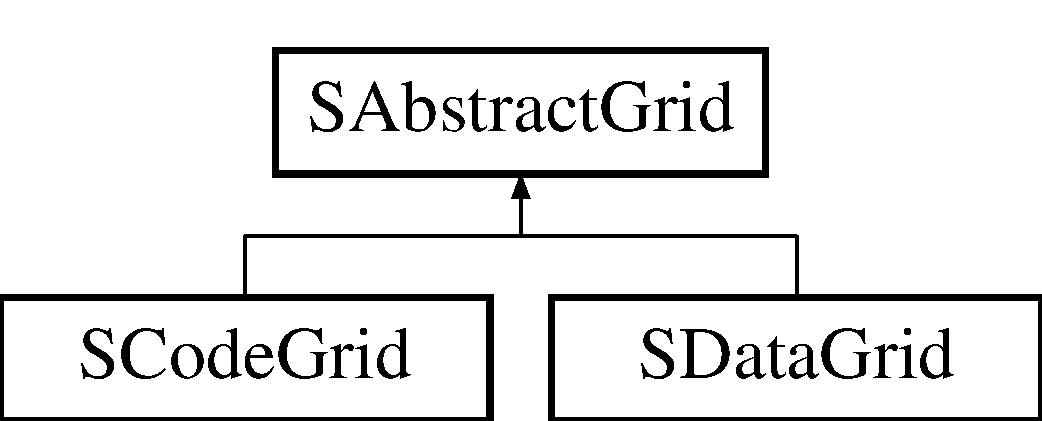
\includegraphics[height=2cm]{classSAbstractGrid}
\end{center}
\end{figure}
\subsection*{Metody publiczne}
\begin{CompactItemize}
\item 
\hyperlink{classSAbstractGrid_2df5b6a5bd2a11d9015104f3dd6afc20}{SAbstractGrid} ()
\item 
virtual \hyperlink{classSAbstractGrid_7391180cba323fbd0d64d23157c8a6a6}{$\sim$SAbstractGrid} ()
\item 
bool \hyperlink{classSAbstractGrid_1e4823efb8b482d44466d8324f63dfb1}{pointInsideGrid} (int, int)
\item 
\hypertarget{classSAbstractGrid_1c10a9c322c321b3fc2c9a5195e817ba}{
virtual int \textbf{\_\-\_\-dev\_\-\_\-transformCharToBinary} (char)=0}
\label{classSAbstractGrid_1c10a9c322c321b3fc2c9a5195e817ba}

\item 
\hypertarget{classSAbstractGrid_6fc913c575c7d1b87b422084129db978}{
virtual char \textbf{\_\-\_\-dev\_\-\_\-transformBinaryToChar} (int)=0}
\label{classSAbstractGrid_6fc913c575c7d1b87b422084129db978}

\item 
\hypertarget{classSAbstractGrid_e36c03b21a96f33d1ace5fd0b1d218f5}{
virtual void \textbf{\_\-\_\-dev\_\-\_\-printConsole} (int, int)=0}
\label{classSAbstractGrid_e36c03b21a96f33d1ace5fd0b1d218f5}

\end{CompactItemize}
\subsection*{Metody chronione}
\begin{CompactItemize}
\item 
virtual void \hyperlink{classSAbstractGrid_919248aad138ffb1c969e73c3e637dcd}{constructGrid} ()=0
\item 
virtual void \hyperlink{classSAbstractGrid_fb63d8cf5210c3606a3b7add19f06833}{destructGrid} ()=0
\item 
virtual int \hyperlink{classSAbstractGrid_d8772e08d58f970d885775cb9682bf6d}{getValueAt} (int, int)=0
\end{CompactItemize}
\subsection*{Atrybuty chronione}
\begin{CompactItemize}
\item 
int \hyperlink{classSAbstractGrid_f0b1916fda47bbd921fc1b5b5abadb72}{size\_\-x}
\item 
int \hyperlink{classSAbstractGrid_b9fddbe2004e7242dff69aa20da8a3c3}{size\_\-y}
\end{CompactItemize}
\subsection*{Przyjaciele}
\begin{CompactItemize}
\item 
\hypertarget{classSAbstractGrid_13f503f5e1b3625e973ac350880b3a31}{
class \hyperlink{classSAbstractGrid_13f503f5e1b3625e973ac350880b3a31}{SCodeMachine}}
\label{classSAbstractGrid_13f503f5e1b3625e973ac350880b3a31}

\item 
\hypertarget{classSAbstractGrid_b064517f75c184bae39efba1df818a12}{
class \hyperlink{classSAbstractGrid_b064517f75c184bae39efba1df818a12}{SDataMachine}}
\label{classSAbstractGrid_b064517f75c184bae39efba1df818a12}

\end{CompactItemize}


\subsection{Opis szczegółowy}
Sbstrakcyjna siatka. 

Siatka jest narzędziem które ułatwia przetrzymywanie pewnych danych w pamięci i udostępnia proste metody wyświetlające te dane na konsolę. Po klasie \hyperlink{classSAbstractGrid}{SAbstractGrid} dziedziczą dwie klasy: \hyperlink{classSCodeGrid}{SCodeGrid} - siatka kodu oraz \hyperlink{classSDataGrid}{SDataGrid} - siatka danych. 

\subsection{Dokumentacja konstruktora i destruktora}
\hypertarget{classSAbstractGrid_2df5b6a5bd2a11d9015104f3dd6afc20}{
\index{SAbstractGrid@{SAbstractGrid}!SAbstractGrid@{SAbstractGrid}}
\index{SAbstractGrid@{SAbstractGrid}!SAbstractGrid@{SAbstractGrid}}
\subsubsection[{SAbstractGrid}]{\setlength{\rightskip}{0pt plus 5cm}SAbstractGrid::SAbstractGrid ()}}
\label{classSAbstractGrid_2df5b6a5bd2a11d9015104f3dd6afc20}


Konstruktor abstrakcyjnej siatki. Nie robi nic szczególnego. \hypertarget{classSAbstractGrid_7391180cba323fbd0d64d23157c8a6a6}{
\index{SAbstractGrid@{SAbstractGrid}!$\sim$SAbstractGrid@{$\sim$SAbstractGrid}}
\index{$\sim$SAbstractGrid@{$\sim$SAbstractGrid}!SAbstractGrid@{SAbstractGrid}}
\subsubsection[{$\sim$SAbstractGrid}]{\setlength{\rightskip}{0pt plus 5cm}SAbstractGrid::$\sim$SAbstractGrid ()\hspace{0.3cm}{\tt  \mbox{[}virtual\mbox{]}}}}
\label{classSAbstractGrid_7391180cba323fbd0d64d23157c8a6a6}


Destruktor abstrakcyjnej siatki. Nie robi nic szczególnego. 

\subsection{Dokumentacja funkcji składowych}
\hypertarget{classSAbstractGrid_919248aad138ffb1c969e73c3e637dcd}{
\index{SAbstractGrid@{SAbstractGrid}!constructGrid@{constructGrid}}
\index{constructGrid@{constructGrid}!SAbstractGrid@{SAbstractGrid}}
\subsubsection[{constructGrid}]{\setlength{\rightskip}{0pt plus 5cm}virtual void SAbstractGrid::constructGrid ()\hspace{0.3cm}{\tt  \mbox{[}protected, pure virtual\mbox{]}}}}
\label{classSAbstractGrid_919248aad138ffb1c969e73c3e637dcd}


Alokuje pamięć pod siatkę. 

Implementowany w \hyperlink{classSCodeGrid_f15ba156433f88a40887e5ba72d9201a}{SCodeGrid} i \hyperlink{classSDataGrid_5af888335764c1ba959b6ef964223b6d}{SDataGrid}.\hypertarget{classSAbstractGrid_fb63d8cf5210c3606a3b7add19f06833}{
\index{SAbstractGrid@{SAbstractGrid}!destructGrid@{destructGrid}}
\index{destructGrid@{destructGrid}!SAbstractGrid@{SAbstractGrid}}
\subsubsection[{destructGrid}]{\setlength{\rightskip}{0pt plus 5cm}virtual void SAbstractGrid::destructGrid ()\hspace{0.3cm}{\tt  \mbox{[}protected, pure virtual\mbox{]}}}}
\label{classSAbstractGrid_fb63d8cf5210c3606a3b7add19f06833}


Dealokuje pamięć przeznaczoną dla siatki. 

Implementowany w \hyperlink{classSCodeGrid_6bd4c1bf841bd09c2ffb2e019c08b4ed}{SCodeGrid} i \hyperlink{classSDataGrid_c9c0ef298fb96c56f9f9796720a41489}{SDataGrid}.\hypertarget{classSAbstractGrid_d8772e08d58f970d885775cb9682bf6d}{
\index{SAbstractGrid@{SAbstractGrid}!getValueAt@{getValueAt}}
\index{getValueAt@{getValueAt}!SAbstractGrid@{SAbstractGrid}}
\subsubsection[{getValueAt}]{\setlength{\rightskip}{0pt plus 5cm}virtual int SAbstractGrid::getValueAt (int, \/  int)\hspace{0.3cm}{\tt  \mbox{[}protected, pure virtual\mbox{]}}}}
\label{classSAbstractGrid_d8772e08d58f970d885775cb9682bf6d}


Zwraca wartość komórki siatki określonej współrzednymi zadanymi parametrami. \begin{Desc}
\item[Zwraca:]wartość komórki siatki wskazanej parametrami \end{Desc}


Implementowany w \hyperlink{classSCodeGrid_c57d52a49a55c91068fe0eb541e721f8}{SCodeGrid} i \hyperlink{classSDataGrid_7f9dd63d74e36731875630a96ea8dd07}{SDataGrid}.\hypertarget{classSAbstractGrid_1e4823efb8b482d44466d8324f63dfb1}{
\index{SAbstractGrid@{SAbstractGrid}!pointInsideGrid@{pointInsideGrid}}
\index{pointInsideGrid@{pointInsideGrid}!SAbstractGrid@{SAbstractGrid}}
\subsubsection[{pointInsideGrid}]{\setlength{\rightskip}{0pt plus 5cm}bool SAbstractGrid::pointInsideGrid (int {\em X}, \/  int {\em Y})}}
\label{classSAbstractGrid_1e4823efb8b482d44466d8324f63dfb1}


Sprawdza czy punkt o współrzędnych zadanych parametrami mieści się w siatce. \begin{Desc}
\item[Parametry:]
\begin{description}
\item[{\em X}]odcięta (współrzędna) \item[{\em Y}]rzędna (współrzędna) \end{description}
\end{Desc}
\begin{Desc}
\item[Zwraca:]czy punkt o zadanych współrzednych mieści się w siatce \end{Desc}


\subsection{Dokumentacja atrybutów składowych}
\hypertarget{classSAbstractGrid_f0b1916fda47bbd921fc1b5b5abadb72}{
\index{SAbstractGrid@{SAbstractGrid}!size\_\-x@{size\_\-x}}
\index{size\_\-x@{size\_\-x}!SAbstractGrid@{SAbstractGrid}}
\subsubsection[{size\_\-x}]{\setlength{\rightskip}{0pt plus 5cm}int {\bf SAbstractGrid::size\_\-x}\hspace{0.3cm}{\tt  \mbox{[}protected\mbox{]}}}}
\label{classSAbstractGrid_f0b1916fda47bbd921fc1b5b5abadb72}


szerokość siatki (rozmiar współrzędnej x) \hypertarget{classSAbstractGrid_b9fddbe2004e7242dff69aa20da8a3c3}{
\index{SAbstractGrid@{SAbstractGrid}!size\_\-y@{size\_\-y}}
\index{size\_\-y@{size\_\-y}!SAbstractGrid@{SAbstractGrid}}
\subsubsection[{size\_\-y}]{\setlength{\rightskip}{0pt plus 5cm}int {\bf SAbstractGrid::size\_\-y}\hspace{0.3cm}{\tt  \mbox{[}protected\mbox{]}}}}
\label{classSAbstractGrid_b9fddbe2004e7242dff69aa20da8a3c3}


wysokość siatki (rozmiar współrzędnej y) 

Dokumentacja dla tej klasy została wygenerowana z plików:\begin{CompactItemize}
\item 
src/core/\hyperlink{sabstractgrid_8h}{sabstractgrid.h}\item 
src/core/\hyperlink{sabstractgrid_8cpp}{sabstractgrid.cpp}\end{CompactItemize}

\hypertarget{classSAbstractMachine}{
\section{Dokumentacja klasy SAbstractMachine}
\label{classSAbstractMachine}\index{SAbstractMachine@{SAbstractMachine}}
}
Abstrakcyjna maszyna.  


{\tt \#include $<$sabstractmachine.h$>$}

Diagram dziedziczenia dla SAbstractMachine:\begin{figure}[H]
\begin{center}
\leavevmode
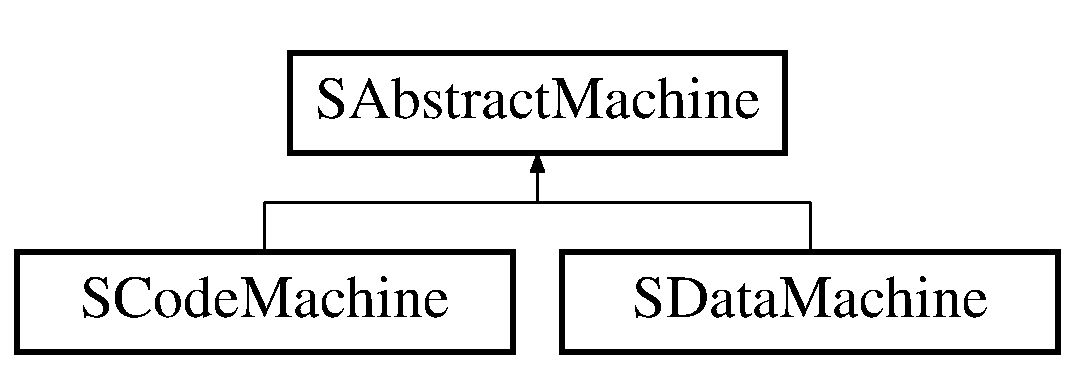
\includegraphics[height=2cm]{classSAbstractMachine}
\end{center}
\end{figure}
\subsection*{Metody publiczne}
\begin{CompactItemize}
\item 
\hyperlink{classSAbstractMachine_f0ffb270de2ea44e89123a873bc5660a}{SAbstractMachine} ()
\item 
\hypertarget{classSAbstractMachine_2c4c79bd629a2961fb520785ce3adf4b}{
virtual \hyperlink{classSAbstractMachine_2c4c79bd629a2961fb520785ce3adf4b}{$\sim$SAbstractMachine} ()}
\label{classSAbstractMachine_2c4c79bd629a2961fb520785ce3adf4b}

\begin{CompactList}\small\item\em Destruktor maszyny abstrakcyjnej. Póki co nie robi nic ciekawego. Nie zajmuje się niszczeniem głowic, tym zajmują się destruktory klas dziedziczących po \hyperlink{classSAbstractMachine}{SAbstractMachine} (\hyperlink{classSCodeMachine}{SCodeMachine}, \hyperlink{classSDataMachine}{SDataMachine}). \item\end{CompactList}\item 
void \hyperlink{classSAbstractMachine_87766a003773869a3438e92739d7c9a1}{clearPointer} ()
\begin{CompactList}\small\item\em ustaw współrzędne głowicy na domyślne \mbox{[}\mbox{[}i kierunek\mbox{]}\mbox{]} \item\end{CompactList}\item 
virtual bool \hyperlink{classSAbstractMachine_72a47b72416e0d2f24fcf36415d37404}{pushPointer} ()=0
\end{CompactItemize}
\subsection*{Atrybuty chronione}
\begin{CompactItemize}
\item 
\hyperlink{classSAbstractPointer}{SAbstractPointer} $\ast$ \hyperlink{classSAbstractMachine_7fb67b2cf326fa3176570ca65c573c79}{pointer}
\item 
\hyperlink{classSAbstractGrid}{SAbstractGrid} $\ast$ \hyperlink{classSAbstractMachine_08b7046c29a7a5f248f324edee91f2dc}{grid}
\end{CompactItemize}


\subsection{Opis szczegółowy}
Abstrakcyjna maszyna. 

Po tej klasie dziedzicza dwie klasy (\hyperlink{classSCodeMachine}{SCodeMachine}, \hyperlink{classSDataMachine}{SDataMachine}, jedne z najważniejszych w projekcie). 

\subsection{Dokumentacja konstruktora i destruktora}
\hypertarget{classSAbstractMachine_f0ffb270de2ea44e89123a873bc5660a}{
\index{SAbstractMachine@{SAbstractMachine}!SAbstractMachine@{SAbstractMachine}}
\index{SAbstractMachine@{SAbstractMachine}!SAbstractMachine@{SAbstractMachine}}
\subsubsection[{SAbstractMachine}]{\setlength{\rightskip}{0pt plus 5cm}SAbstractMachine::SAbstractMachine ()}}
\label{classSAbstractMachine_f0ffb270de2ea44e89123a873bc5660a}


Konstruktor maszyny abstrakcyjnej. Póki co nie robi nic ciekawego. Nie zajmuje się tworzeniem głowic, tym zajmują się konstruktory klas dziedziczących po \hyperlink{classSAbstractMachine}{SAbstractMachine} (\hyperlink{classSCodeMachine}{SCodeMachine}, \hyperlink{classSDataMachine}{SDataMachine}). 

\subsection{Dokumentacja funkcji składowych}
\hypertarget{classSAbstractMachine_87766a003773869a3438e92739d7c9a1}{
\index{SAbstractMachine@{SAbstractMachine}!clearPointer@{clearPointer}}
\index{clearPointer@{clearPointer}!SAbstractMachine@{SAbstractMachine}}
\subsubsection[{clearPointer}]{\setlength{\rightskip}{0pt plus 5cm}void SAbstractMachine::clearPointer ()}}
\label{classSAbstractMachine_87766a003773869a3438e92739d7c9a1}


ustaw współrzędne głowicy na domyślne \mbox{[}\mbox{[}i kierunek\mbox{]}\mbox{]} 

Ustawia współrzędne głowicy na wartości domyślne. Wewnątrz klasy \hyperlink{classSAbstractMachine}{SAbstractMachine} nie zostaje tworzony żaden obiekt głowicy (ani \hyperlink{classSCodeImagePointer}{SCodeImagePointer}, ani \hyperlink{classSDataImagePointer}{SDataImagePointer}). Są one tworzone w konstruktorach klas dziedziczących po \hyperlink{classSAbstractMachine}{SAbstractMachine}, czyli odpowiednio: \hyperlink{classSCodeMachine}{SCodeMachine} lub \hyperlink{classSDataMachine}{SDataMachine}. Jakoże obie głowice dziedziczą po klasie \hyperlink{classSAbstractPointer}{SAbstractPointer} (zdefiniowane są w niej współdzędne), możliwe jest użycie wskaźnika na głowicę (teoretycznie bez jej utworzenia, przynajmniej w tej klasie) \hypertarget{classSAbstractMachine_72a47b72416e0d2f24fcf36415d37404}{
\index{SAbstractMachine@{SAbstractMachine}!pushPointer@{pushPointer}}
\index{pushPointer@{pushPointer}!SAbstractMachine@{SAbstractMachine}}
\subsubsection[{pushPointer}]{\setlength{\rightskip}{0pt plus 5cm}virtual bool SAbstractMachine::pushPointer ()\hspace{0.3cm}{\tt  \mbox{[}pure virtual\mbox{]}}}}
\label{classSAbstractMachine_72a47b72416e0d2f24fcf36415d37404}


Przesuwa głowicę o jedną komórkę w bieżącym kierunku. 

Implementowany w \hyperlink{classSCodeMachine_69a97f71f2a16f69f9daca1bf8433964}{SCodeMachine} i \hyperlink{classSDataMachine_10eb8f56cf6235455a26c5c673b8fe15}{SDataMachine}.

\subsection{Dokumentacja atrybutów składowych}
\hypertarget{classSAbstractMachine_08b7046c29a7a5f248f324edee91f2dc}{
\index{SAbstractMachine@{SAbstractMachine}!grid@{grid}}
\index{grid@{grid}!SAbstractMachine@{SAbstractMachine}}
\subsubsection[{grid}]{\setlength{\rightskip}{0pt plus 5cm}{\bf SAbstractGrid}$\ast$ {\bf SAbstractMachine::grid}\hspace{0.3cm}{\tt  \mbox{[}protected\mbox{]}}}}
\label{classSAbstractMachine_08b7046c29a7a5f248f324edee91f2dc}


Siatka maszyny. Maszyna kodu ma swoją siatkę, a maszyna danych swoją. \hypertarget{classSAbstractMachine_7fb67b2cf326fa3176570ca65c573c79}{
\index{SAbstractMachine@{SAbstractMachine}!pointer@{pointer}}
\index{pointer@{pointer}!SAbstractMachine@{SAbstractMachine}}
\subsubsection[{pointer}]{\setlength{\rightskip}{0pt plus 5cm}{\bf SAbstractPointer}$\ast$ {\bf SAbstractMachine::pointer}\hspace{0.3cm}{\tt  \mbox{[}protected\mbox{]}}}}
\label{classSAbstractMachine_7fb67b2cf326fa3176570ca65c573c79}


Głowica maszyny. Maszyna kodu ma swoją głowicę, a maszyna danych swoją. 

Dokumentacja dla tej klasy została wygenerowana z plików:\begin{CompactItemize}
\item 
src/core/\hyperlink{sabstractmachine_8h}{sabstractmachine.h}\item 
src/core/\hyperlink{sabstractmachine_8cpp}{sabstractmachine.cpp}\end{CompactItemize}

\hypertarget{classSAbstractPointer}{
\section{Dokumentacja klasy SAbstractPointer}
\label{classSAbstractPointer}\index{SAbstractPointer@{SAbstractPointer}}
}
abstrakcyjna głowica maszyn  


{\tt \#include $<$sabstractpointer.h$>$}

Diagram dziedziczenia dla SAbstractPointer:\begin{figure}[H]
\begin{center}
\leavevmode
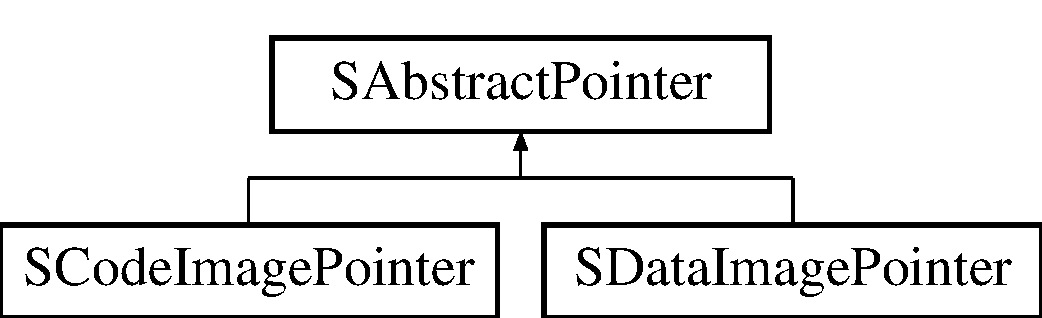
\includegraphics[height=2cm]{classSAbstractPointer}
\end{center}
\end{figure}
\subsection*{Metody publiczne}
\begin{CompactItemize}
\item 
\hyperlink{classSAbstractPointer_9281c3dba0da68460fa87bd17bd768b4}{SAbstractPointer} ()
\item 
virtual \hyperlink{classSAbstractPointer_9973354ecf610b3d48170dd70f0b22ce}{$\sim$SAbstractPointer} ()
\item 
\hypertarget{classSAbstractPointer_bb15625597bfe9f3927cdc360214bc55}{
void \textbf{clear} ()}
\label{classSAbstractPointer_bb15625597bfe9f3927cdc360214bc55}

\item 
\hypertarget{classSAbstractPointer_c4655988c5ae9f94a00e3ccd0ed14863}{
void \textbf{moveForward} (int)}
\label{classSAbstractPointer_c4655988c5ae9f94a00e3ccd0ed14863}

\item 
\hypertarget{classSAbstractPointer_5d7349c25205be738561fa791a77a3b8}{
std::string \textbf{\_\-\_\-dev\_\-\_\-transformBinaryDirectionToString} (\hyperlink{senums_8h_039d4115103dc22e0555ecc968fecbf0}{SDirections})}
\label{classSAbstractPointer_5d7349c25205be738561fa791a77a3b8}

\item 
\hypertarget{classSAbstractPointer_3faa92c6a0de5ea971a7d32ceb51980f}{
void \textbf{\_\-\_\-dev\_\-\_\-printConsoleCoords} ()}
\label{classSAbstractPointer_3faa92c6a0de5ea971a7d32ceb51980f}

\item 
\hypertarget{classSAbstractPointer_2a94015a951c9a7181d8aad4d4a356d3}{
int \textbf{\_\-\_\-dev\_\-\_\-getCoordX} ()}
\label{classSAbstractPointer_2a94015a951c9a7181d8aad4d4a356d3}

\item 
\hypertarget{classSAbstractPointer_413be96bf36c59e49c00b5ae0c297c90}{
int \textbf{\_\-\_\-dev\_\-\_\-getCoordY} ()}
\label{classSAbstractPointer_413be96bf36c59e49c00b5ae0c297c90}

\end{CompactItemize}
\subsection*{Metody chronione}
\begin{CompactItemize}
\item 
\hypertarget{classSAbstractPointer_0e44b215ff78c8315a4fc4dc12cd4049}{
int \textbf{getCoordX} ()}
\label{classSAbstractPointer_0e44b215ff78c8315a4fc4dc12cd4049}

\item 
\hypertarget{classSAbstractPointer_0226e83b6f838f3ee8491915b9ebab74}{
int \textbf{getCoordY} ()}
\label{classSAbstractPointer_0226e83b6f838f3ee8491915b9ebab74}

\item 
\hypertarget{classSAbstractPointer_e1b27cb6a14cbf77e4499d8ca1ae7c90}{
void \textbf{setDirection} (\hyperlink{senums_8h_039d4115103dc22e0555ecc968fecbf0}{SDirections})}
\label{classSAbstractPointer_e1b27cb6a14cbf77e4499d8ca1ae7c90}

\end{CompactItemize}
\subsection*{Atrybuty chronione}
\begin{CompactItemize}
\item 
\hypertarget{classSAbstractPointer_f4a22efc5fe4922cfe61ac8d849d6849}{
int \textbf{coord\_\-x}}
\label{classSAbstractPointer_f4a22efc5fe4922cfe61ac8d849d6849}

\item 
\hypertarget{classSAbstractPointer_8804aa2589dc17c401c438a2f4a1c489}{
int \textbf{coord\_\-y}}
\label{classSAbstractPointer_8804aa2589dc17c401c438a2f4a1c489}

\item 
\hypertarget{classSAbstractPointer_6e8b50c6806f43a8b29596c8899db4f2}{
\hyperlink{senums_8h_039d4115103dc22e0555ecc968fecbf0}{SDirections} \textbf{direction}}
\label{classSAbstractPointer_6e8b50c6806f43a8b29596c8899db4f2}

\end{CompactItemize}
\subsection*{Przyjaciele}
\begin{CompactItemize}
\item 
\hypertarget{classSAbstractPointer_13f503f5e1b3625e973ac350880b3a31}{
class \hyperlink{classSAbstractPointer_13f503f5e1b3625e973ac350880b3a31}{SCodeMachine}}
\label{classSAbstractPointer_13f503f5e1b3625e973ac350880b3a31}

\item 
\hypertarget{classSAbstractPointer_b064517f75c184bae39efba1df818a12}{
class \hyperlink{classSAbstractPointer_b064517f75c184bae39efba1df818a12}{SDataMachine}}
\label{classSAbstractPointer_b064517f75c184bae39efba1df818a12}

\end{CompactItemize}


\subsection{Opis szczegółowy}
abstrakcyjna głowica maszyn 

Głowice są wykorzystywane przez maszyny danych i kodu 

\subsection{Dokumentacja konstruktora i destruktora}
\hypertarget{classSAbstractPointer_9281c3dba0da68460fa87bd17bd768b4}{
\index{SAbstractPointer@{SAbstractPointer}!SAbstractPointer@{SAbstractPointer}}
\index{SAbstractPointer@{SAbstractPointer}!SAbstractPointer@{SAbstractPointer}}
\subsubsection[{SAbstractPointer}]{\setlength{\rightskip}{0pt plus 5cm}SAbstractPointer::SAbstractPointer ()}}
\label{classSAbstractPointer_9281c3dba0da68460fa87bd17bd768b4}


Konstruktor głowicy abstrakcyjnej. Ustala atrybuty głowicy (współrzędne, kierunek poruszania itp.) na wartości domyślne. \hypertarget{classSAbstractPointer_9973354ecf610b3d48170dd70f0b22ce}{
\index{SAbstractPointer@{SAbstractPointer}!$\sim$SAbstractPointer@{$\sim$SAbstractPointer}}
\index{$\sim$SAbstractPointer@{$\sim$SAbstractPointer}!SAbstractPointer@{SAbstractPointer}}
\subsubsection[{$\sim$SAbstractPointer}]{\setlength{\rightskip}{0pt plus 5cm}SAbstractPointer::$\sim$SAbstractPointer ()\hspace{0.3cm}{\tt  \mbox{[}virtual\mbox{]}}}}
\label{classSAbstractPointer_9973354ecf610b3d48170dd70f0b22ce}


Destruktor głowicy abstrakcyjnej. Nie robi nic szczególnego. 

Dokumentacja dla tej klasy została wygenerowana z plików:\begin{CompactItemize}
\item 
src/core/\hyperlink{sabstractpointer_8h}{sabstractpointer.h}\item 
src/core/\hyperlink{sabstractpointer_8cpp}{sabstractpointer.cpp}\end{CompactItemize}

\hypertarget{classSCodeGrid}{
\section{Dokumentacja klasy SCodeGrid}
\label{classSCodeGrid}\index{SCodeGrid@{SCodeGrid}}
}
siatka kodu  


{\tt \#include $<$scodegrid.h$>$}

Diagram dziedziczenia dla SCodeGrid:\begin{figure}[H]
\begin{center}
\leavevmode
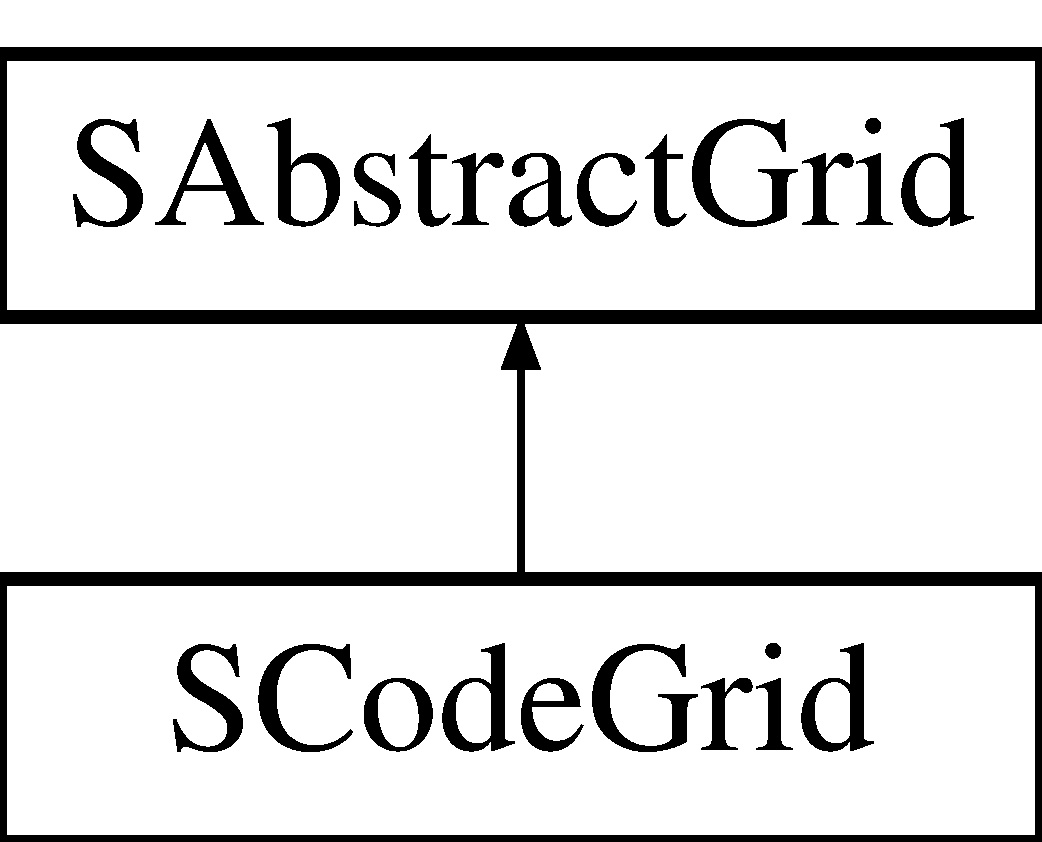
\includegraphics[height=2cm]{classSCodeGrid}
\end{center}
\end{figure}
\subsection*{Metody publiczne}
\begin{CompactItemize}
\item 
\hyperlink{classSCodeGrid_e430762ac9855cd60f8d5a57c46428b9}{SCodeGrid} (std::string, \hyperlink{senums_8h_1a2ae45552936d27425f99e1c187b043}{SCodeTypes})
\item 
\hyperlink{classSCodeGrid_c150afdd8f27785b5ddf5669a4d90332}{$\sim$SCodeGrid} ()
\item 
\hypertarget{classSCodeGrid_c57d52a49a55c91068fe0eb541e721f8}{
int \textbf{getValueAt} (int, int)}
\label{classSCodeGrid_c57d52a49a55c91068fe0eb541e721f8}

\item 
\hypertarget{classSCodeGrid_c01feeae87539b97aed07d67b975f174}{
void \textbf{\_\-\_\-dev\_\-\_\-printConsole} (int, int)}
\label{classSCodeGrid_c01feeae87539b97aed07d67b975f174}

\item 
\hypertarget{classSCodeGrid_c5754181e1266e23935d84f3beeb5979}{
int \textbf{\_\-\_\-dev\_\-\_\-transformCharToBinary} (char)}
\label{classSCodeGrid_c5754181e1266e23935d84f3beeb5979}

\item 
\hypertarget{classSCodeGrid_75d1d340ee3c5704527e793f2e71e93b}{
char \textbf{\_\-\_\-dev\_\-\_\-transformBinaryToChar} (int)}
\label{classSCodeGrid_75d1d340ee3c5704527e793f2e71e93b}

\end{CompactItemize}
\subsection*{Metody chronione}
\begin{CompactItemize}
\item 
int \hyperlink{classSCodeGrid_46ed88ad7346788efb14c40cbd836981}{readFromFile} (std::string)
\item 
\hypertarget{classSCodeGrid_f15ba156433f88a40887e5ba72d9201a}{
void \textbf{constructGrid} ()}
\label{classSCodeGrid_f15ba156433f88a40887e5ba72d9201a}

\item 
\hypertarget{classSCodeGrid_6bd4c1bf841bd09c2ffb2e019c08b4ed}{
void \textbf{destructGrid} ()}
\label{classSCodeGrid_6bd4c1bf841bd09c2ffb2e019c08b4ed}

\end{CompactItemize}
\subsection*{Atrybuty chronione}
\begin{CompactItemize}
\item 
\hypertarget{classSCodeGrid_445b4bd8cca6ddb7100afa621f5722b0}{
\hyperlink{senums_8h_b1c3fa9dccd3f8afa81e14a98d9a7d1e}{SInstructions} $\ast$$\ast$ \textbf{instruction\_\-grid}}
\label{classSCodeGrid_445b4bd8cca6ddb7100afa621f5722b0}

\end{CompactItemize}


\subsection{Opis szczegółowy}
siatka kodu 

2 cele:

\begin{itemize}
\item testowanie (development)\item nakładanie na obrazek siatki kodu (celem stworzenia obrazka zawierającego program) \end{itemize}


\subsection{Dokumentacja konstruktora i destruktora}
\hypertarget{classSCodeGrid_e430762ac9855cd60f8d5a57c46428b9}{
\index{SCodeGrid@{SCodeGrid}!SCodeGrid@{SCodeGrid}}
\index{SCodeGrid@{SCodeGrid}!SCodeGrid@{SCodeGrid}}
\subsubsection[{SCodeGrid}]{\setlength{\rightskip}{0pt plus 5cm}SCodeGrid::SCodeGrid (std::string {\em filename}, \/  {\bf SCodeTypes} {\em CODE\_\-TYPE})}}
\label{classSCodeGrid_e430762ac9855cd60f8d5a57c46428b9}


Konstruktor siatki kodu. \hypertarget{classSCodeGrid_c150afdd8f27785b5ddf5669a4d90332}{
\index{SCodeGrid@{SCodeGrid}!$\sim$SCodeGrid@{$\sim$SCodeGrid}}
\index{$\sim$SCodeGrid@{$\sim$SCodeGrid}!SCodeGrid@{SCodeGrid}}
\subsubsection[{$\sim$SCodeGrid}]{\setlength{\rightskip}{0pt plus 5cm}SCodeGrid::$\sim$SCodeGrid ()}}
\label{classSCodeGrid_c150afdd8f27785b5ddf5669a4d90332}


Destruktor siatki kodu. 

\subsection{Dokumentacja funkcji składowych}
\hypertarget{classSCodeGrid_46ed88ad7346788efb14c40cbd836981}{
\index{SCodeGrid@{SCodeGrid}!readFromFile@{readFromFile}}
\index{readFromFile@{readFromFile}!SCodeGrid@{SCodeGrid}}
\subsubsection[{readFromFile}]{\setlength{\rightskip}{0pt plus 5cm}int SCodeGrid::readFromFile (std::string {\em filename})\hspace{0.3cm}{\tt  \mbox{[}protected\mbox{]}}}}
\label{classSCodeGrid_46ed88ad7346788efb14c40cbd836981}


\begin{Desc}
\item[Zwraca:]kod błędu: 0: ok 1: nie ma takiego pliku 2: błędny format wejścia \end{Desc}


Dokumentacja dla tej klasy została wygenerowana z plików:\begin{CompactItemize}
\item 
src/core/\hyperlink{scodegrid_8h}{scodegrid.h}\item 
src/core/\hyperlink{scodegrid_8cpp}{scodegrid.cpp}\end{CompactItemize}

\hypertarget{classSCodeImagePointer}{
\section{Dokumentacja klasy SCodeImagePointer}
\label{classSCodeImagePointer}\index{SCodeImagePointer@{SCodeImagePointer}}
}
głowica maszyny obsługująca obraz kodu  


{\tt \#include $<$scodeimagepointer.h$>$}

Diagram dziedziczenia dla SCodeImagePointer:\begin{figure}[H]
\begin{center}
\leavevmode
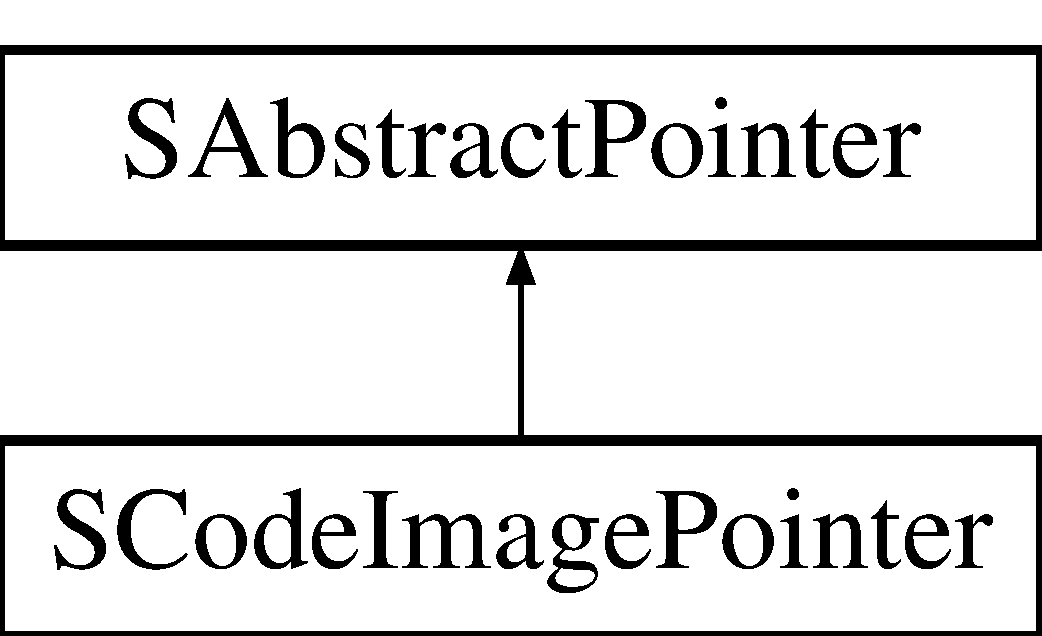
\includegraphics[height=2cm]{classSCodeImagePointer}
\end{center}
\end{figure}
\subsection*{Metody publiczne}
\begin{CompactItemize}
\item 
\hyperlink{classSCodeImagePointer_bcef321f6fed2e37ca660978d86a3ecb}{SCodeImagePointer} ()
\item 
\hyperlink{classSCodeImagePointer_65cc13e9ddfa6b12ff7ef24f658b5015}{$\sim$SCodeImagePointer} ()
\item 
void \hyperlink{classSCodeImagePointer_01367459d424aa6155f98c8cd8b930d5}{turnUp} ()
\item 
void \hyperlink{classSCodeImagePointer_fd353f45c3b71bfd402bbef5f9248752}{turnDown} ()
\item 
void \hyperlink{classSCodeImagePointer_a3e17be0016265dfb389d64fe63c24ac}{turnLeft} ()
\item 
void \hyperlink{classSCodeImagePointer_352a2e1c0039812322ce48e183e246de}{turnRight} ()
\end{CompactItemize}


\subsection{Opis szczegółowy}
głowica maszyny obsługująca obraz kodu 

Obiekt klasy \hyperlink{classSCodeImagePointer}{SCodeImagePointer} jest swoistym wskaźnikiem na daną komórkę obrazu kodu. Maszyna danych (\hyperlink{classSCodeMachine}{SCodeMachine}) wykorzystuje głowicę, by dzięki niej odczytywać wartości z obrazu kodu (SCodeImage) oraz by na tym obrazie zapisywać nowe wartości. 

\subsection{Dokumentacja konstruktora i destruktora}
\hypertarget{classSCodeImagePointer_bcef321f6fed2e37ca660978d86a3ecb}{
\index{SCodeImagePointer@{SCodeImagePointer}!SCodeImagePointer@{SCodeImagePointer}}
\index{SCodeImagePointer@{SCodeImagePointer}!SCodeImagePointer@{SCodeImagePointer}}
\subsubsection[{SCodeImagePointer}]{\setlength{\rightskip}{0pt plus 5cm}SCodeImagePointer::SCodeImagePointer ()}}
\label{classSCodeImagePointer_bcef321f6fed2e37ca660978d86a3ecb}


Konstruktor głowicy obrazu kodu. Nie robi nic szczególnego. \hypertarget{classSCodeImagePointer_65cc13e9ddfa6b12ff7ef24f658b5015}{
\index{SCodeImagePointer@{SCodeImagePointer}!$\sim$SCodeImagePointer@{$\sim$SCodeImagePointer}}
\index{$\sim$SCodeImagePointer@{$\sim$SCodeImagePointer}!SCodeImagePointer@{SCodeImagePointer}}
\subsubsection[{$\sim$SCodeImagePointer}]{\setlength{\rightskip}{0pt plus 5cm}SCodeImagePointer::$\sim$SCodeImagePointer ()}}
\label{classSCodeImagePointer_65cc13e9ddfa6b12ff7ef24f658b5015}


Destruktor głowicy obrazu kodu. Nie robi nic szczególnego. 

\subsection{Dokumentacja funkcji składowych}
\hypertarget{classSCodeImagePointer_fd353f45c3b71bfd402bbef5f9248752}{
\index{SCodeImagePointer@{SCodeImagePointer}!turnDown@{turnDown}}
\index{turnDown@{turnDown}!SCodeImagePointer@{SCodeImagePointer}}
\subsubsection[{turnDown}]{\setlength{\rightskip}{0pt plus 5cm}void SCodeImagePointer::turnDown ()}}
\label{classSCodeImagePointer_fd353f45c3b71bfd402bbef5f9248752}


Ustawia kierunek poruszania się głowicy kodu na dół. \hypertarget{classSCodeImagePointer_a3e17be0016265dfb389d64fe63c24ac}{
\index{SCodeImagePointer@{SCodeImagePointer}!turnLeft@{turnLeft}}
\index{turnLeft@{turnLeft}!SCodeImagePointer@{SCodeImagePointer}}
\subsubsection[{turnLeft}]{\setlength{\rightskip}{0pt plus 5cm}void SCodeImagePointer::turnLeft ()}}
\label{classSCodeImagePointer_a3e17be0016265dfb389d64fe63c24ac}


Ustawia kierunek poruszania się głowicy kodu na lewo. \hypertarget{classSCodeImagePointer_352a2e1c0039812322ce48e183e246de}{
\index{SCodeImagePointer@{SCodeImagePointer}!turnRight@{turnRight}}
\index{turnRight@{turnRight}!SCodeImagePointer@{SCodeImagePointer}}
\subsubsection[{turnRight}]{\setlength{\rightskip}{0pt plus 5cm}void SCodeImagePointer::turnRight ()}}
\label{classSCodeImagePointer_352a2e1c0039812322ce48e183e246de}


Ustawia kierunek poruszania się głowicy kodu na prawo. \hypertarget{classSCodeImagePointer_01367459d424aa6155f98c8cd8b930d5}{
\index{SCodeImagePointer@{SCodeImagePointer}!turnUp@{turnUp}}
\index{turnUp@{turnUp}!SCodeImagePointer@{SCodeImagePointer}}
\subsubsection[{turnUp}]{\setlength{\rightskip}{0pt plus 5cm}void SCodeImagePointer::turnUp ()}}
\label{classSCodeImagePointer_01367459d424aa6155f98c8cd8b930d5}


Ustawia kierunek poruszania się głowicy kodu na górę. 

Dokumentacja dla tej klasy została wygenerowana z plików:\begin{CompactItemize}
\item 
src/core/\hyperlink{scodeimagepointer_8h}{scodeimagepointer.h}\item 
src/core/\hyperlink{scodeimagepointer_8cpp}{scodeimagepointer.cpp}\end{CompactItemize}

\hypertarget{classSCodeMachine}{
\section{Dokumentacja klasy SCodeMachine}
\label{classSCodeMachine}\index{SCodeMachine@{SCodeMachine}}
}
maszyna danych, obsługująca obraz danych  


{\tt \#include $<$scodemachine.h$>$}

Diagram dziedziczenia dla SCodeMachine:\begin{figure}[H]
\begin{center}
\leavevmode
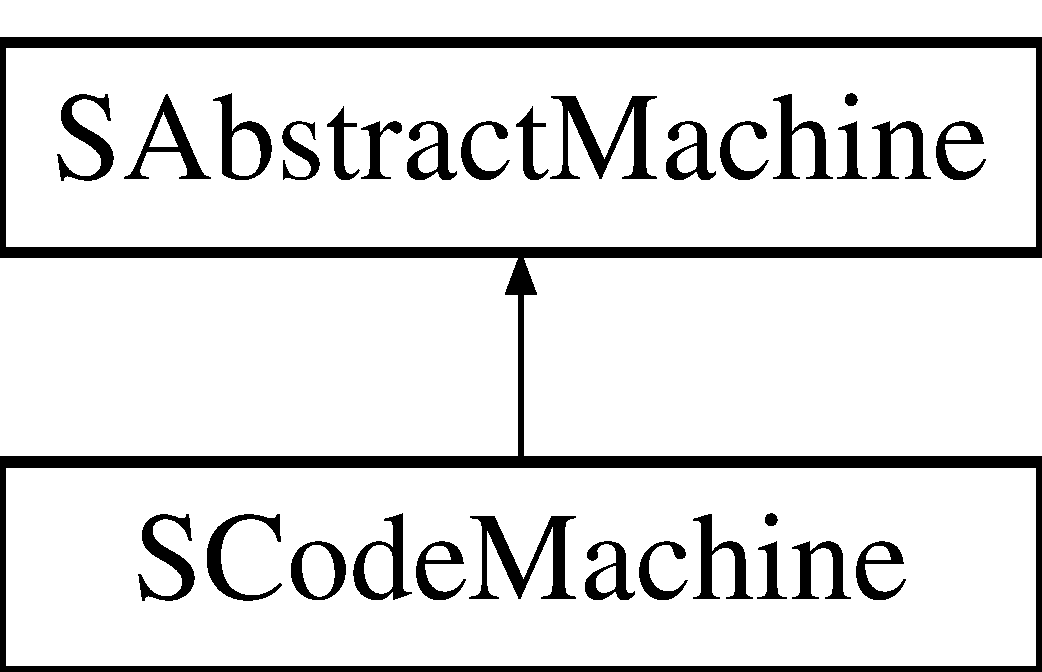
\includegraphics[height=2cm]{classSCodeMachine}
\end{center}
\end{figure}
\subsection*{Metody publiczne}
\begin{CompactItemize}
\item 
\hyperlink{classSCodeMachine_bb85f472be7c8e2112bbe5d6643f99b7}{SCodeMachine} (\hyperlink{senums_8h_1a2ae45552936d27425f99e1c187b043}{SCodeTypes})
\item 
\hyperlink{classSCodeMachine_67d39a3662fc2640aa506a581766a9b8}{$\sim$SCodeMachine} ()
\item 
void \hyperlink{classSCodeMachine_4a2d7edca4db9e3bd8942abc13f6c8ec}{setVerbosity} (bool)
\item 
\hyperlink{senums_8h_b1c3fa9dccd3f8afa81e14a98d9a7d1e}{SInstructions} \hyperlink{classSCodeMachine_3c851e80ec35cbebeb78ec8ceed8c5ca}{getPointedInstruction} ()
\item 
bool \hyperlink{classSCodeMachine_69a97f71f2a16f69f9daca1bf8433964}{pushPointer} ()
\item 
void \hyperlink{classSCodeMachine_d8415a221140a08a9383a595336cdf69}{executeTurnLeft} ()
\item 
void \hyperlink{classSCodeMachine_d48065e7bf42eef9e3a0f81fbb17f301}{executeTurnRight} ()
\item 
void \hyperlink{classSCodeMachine_f2867d02414db096844e4801f9895650}{executeTurnUp} ()
\item 
void \hyperlink{classSCodeMachine_26b7ba8981d08d594b0c37617aa85277}{executeTurnDown} ()
\item 
\hypertarget{classSCodeMachine_f83465e2ab7065c7b386a189d57ae9ab}{
void \textbf{\_\-\_\-dev\_\-\_\-readGridFromTextFile} (std::string)}
\label{classSCodeMachine_f83465e2ab7065c7b386a189d57ae9ab}

\item 
\hypertarget{classSCodeMachine_c9345e02c8383585cf1738c653f83cfd}{
void \textbf{\_\-\_\-dev\_\-\_\-destroyGrid} ()}
\label{classSCodeMachine_c9345e02c8383585cf1738c653f83cfd}

\item 
void \hyperlink{classSCodeMachine_29892f8f026e8dcd71ec99b9c593e022}{\_\-\_\-dev\_\-\_\-printConsole} ()
\item 
void \hyperlink{classSCodeMachine_b4c8492fda9fe21cc2620ede3630d852}{\_\-\_\-dev\_\-\_\-printPointer} ()
\item 
\hypertarget{classSCodeMachine_0ea93dafdabff0ff080a24b6c8ef9ea1}{
void \textbf{\_\-\_\-dev\_\-\_\-printGrid} ()}
\label{classSCodeMachine_0ea93dafdabff0ff080a24b6c8ef9ea1}

\item 
void \hyperlink{classSCodeMachine_6a725d341bffacccb53431f88c62b713}{\_\-\_\-dev\_\-\_\-printPointedInstruction} ()
\end{CompactItemize}


\subsection{Opis szczegółowy}
maszyna danych, obsługująca obraz danych 

Obiekt klasy \hyperlink{classSCodeMachine}{SCodeMachine} to tzw. \char`\"{}maszyna kodu\char`\"{} która obsługuje dane programu wykonywanego przez wirtualną maszynę Salvadora. Maszyna ta posiada sam obraz danych, będący graficzną reprezentacją danych wykonywanego programu. 

\subsection{Dokumentacja konstruktora i destruktora}
\hypertarget{classSCodeMachine_bb85f472be7c8e2112bbe5d6643f99b7}{
\index{SCodeMachine@{SCodeMachine}!SCodeMachine@{SCodeMachine}}
\index{SCodeMachine@{SCodeMachine}!SCodeMachine@{SCodeMachine}}
\subsubsection[{SCodeMachine}]{\setlength{\rightskip}{0pt plus 5cm}SCodeMachine::SCodeMachine ({\bf SCodeTypes} {\em CODE\_\-TYPE})}}
\label{classSCodeMachine_bb85f472be7c8e2112bbe5d6643f99b7}


Konstruktor maszyny kodu. Tworzy obiekty głowicy obrazu kodu oraz sam obraz kodu. \hypertarget{classSCodeMachine_67d39a3662fc2640aa506a581766a9b8}{
\index{SCodeMachine@{SCodeMachine}!$\sim$SCodeMachine@{$\sim$SCodeMachine}}
\index{$\sim$SCodeMachine@{$\sim$SCodeMachine}!SCodeMachine@{SCodeMachine}}
\subsubsection[{$\sim$SCodeMachine}]{\setlength{\rightskip}{0pt plus 5cm}SCodeMachine::$\sim$SCodeMachine ()}}
\label{classSCodeMachine_67d39a3662fc2640aa506a581766a9b8}


Destruktor maszyny kodu. Niszczy obiekty głowicy obrazu kodu oraz sam obraz kodu. 

\subsection{Dokumentacja funkcji składowych}
\hypertarget{classSCodeMachine_29892f8f026e8dcd71ec99b9c593e022}{
\index{SCodeMachine@{SCodeMachine}!\_\-\_\-dev\_\-\_\-printConsole@{\_\-\_\-dev\_\-\_\-printConsole}}
\index{\_\-\_\-dev\_\-\_\-printConsole@{\_\-\_\-dev\_\-\_\-printConsole}!SCodeMachine@{SCodeMachine}}
\subsubsection[{\_\-\_\-dev\_\-\_\-printConsole}]{\setlength{\rightskip}{0pt plus 5cm}void SCodeMachine::\_\-\_\-dev\_\-\_\-printConsole ()}}
\label{classSCodeMachine_29892f8f026e8dcd71ec99b9c593e022}


METODA TESTOWA. Wyświetla informacje o maszynie kodu. \hypertarget{classSCodeMachine_6a725d341bffacccb53431f88c62b713}{
\index{SCodeMachine@{SCodeMachine}!\_\-\_\-dev\_\-\_\-printPointedInstruction@{\_\-\_\-dev\_\-\_\-printPointedInstruction}}
\index{\_\-\_\-dev\_\-\_\-printPointedInstruction@{\_\-\_\-dev\_\-\_\-printPointedInstruction}!SCodeMachine@{SCodeMachine}}
\subsubsection[{\_\-\_\-dev\_\-\_\-printPointedInstruction}]{\setlength{\rightskip}{0pt plus 5cm}void SCodeMachine::\_\-\_\-dev\_\-\_\-printPointedInstruction ()}}
\label{classSCodeMachine_6a725d341bffacccb53431f88c62b713}


METODA TESTOWA. Wyświetla nazwę wskazywanje przez głowicę instrukcji. \hypertarget{classSCodeMachine_b4c8492fda9fe21cc2620ede3630d852}{
\index{SCodeMachine@{SCodeMachine}!\_\-\_\-dev\_\-\_\-printPointer@{\_\-\_\-dev\_\-\_\-printPointer}}
\index{\_\-\_\-dev\_\-\_\-printPointer@{\_\-\_\-dev\_\-\_\-printPointer}!SCodeMachine@{SCodeMachine}}
\subsubsection[{\_\-\_\-dev\_\-\_\-printPointer}]{\setlength{\rightskip}{0pt plus 5cm}void SCodeMachine::\_\-\_\-dev\_\-\_\-printPointer ()}}
\label{classSCodeMachine_b4c8492fda9fe21cc2620ede3630d852}


METODA TESTOWA. Wyświetla informacje o głowicy maszyny. \hypertarget{classSCodeMachine_26b7ba8981d08d594b0c37617aa85277}{
\index{SCodeMachine@{SCodeMachine}!executeTurnDown@{executeTurnDown}}
\index{executeTurnDown@{executeTurnDown}!SCodeMachine@{SCodeMachine}}
\subsubsection[{executeTurnDown}]{\setlength{\rightskip}{0pt plus 5cm}void SCodeMachine::executeTurnDown ()}}
\label{classSCodeMachine_26b7ba8981d08d594b0c37617aa85277}


Wykonuje instrukcję Salvadora SKRĘĆ GŁOWICE KODU W DÓŁ. \hypertarget{classSCodeMachine_d8415a221140a08a9383a595336cdf69}{
\index{SCodeMachine@{SCodeMachine}!executeTurnLeft@{executeTurnLeft}}
\index{executeTurnLeft@{executeTurnLeft}!SCodeMachine@{SCodeMachine}}
\subsubsection[{executeTurnLeft}]{\setlength{\rightskip}{0pt plus 5cm}void SCodeMachine::executeTurnLeft ()}}
\label{classSCodeMachine_d8415a221140a08a9383a595336cdf69}


Wykonuje instrukcję Salvadora SKRĘĆ GŁOWICE KODU W LEWO. \hypertarget{classSCodeMachine_d48065e7bf42eef9e3a0f81fbb17f301}{
\index{SCodeMachine@{SCodeMachine}!executeTurnRight@{executeTurnRight}}
\index{executeTurnRight@{executeTurnRight}!SCodeMachine@{SCodeMachine}}
\subsubsection[{executeTurnRight}]{\setlength{\rightskip}{0pt plus 5cm}void SCodeMachine::executeTurnRight ()}}
\label{classSCodeMachine_d48065e7bf42eef9e3a0f81fbb17f301}


Wykonuje instrukcję Salvadora SKRĘĆ GŁOWICE KODU W PRAWO. \hypertarget{classSCodeMachine_f2867d02414db096844e4801f9895650}{
\index{SCodeMachine@{SCodeMachine}!executeTurnUp@{executeTurnUp}}
\index{executeTurnUp@{executeTurnUp}!SCodeMachine@{SCodeMachine}}
\subsubsection[{executeTurnUp}]{\setlength{\rightskip}{0pt plus 5cm}void SCodeMachine::executeTurnUp ()}}
\label{classSCodeMachine_f2867d02414db096844e4801f9895650}


Wykonuje instrukcję Salvadora SKRĘĆ GŁOWICE KODU W GÓRĘ. \hypertarget{classSCodeMachine_3c851e80ec35cbebeb78ec8ceed8c5ca}{
\index{SCodeMachine@{SCodeMachine}!getPointedInstruction@{getPointedInstruction}}
\index{getPointedInstruction@{getPointedInstruction}!SCodeMachine@{SCodeMachine}}
\subsubsection[{getPointedInstruction}]{\setlength{\rightskip}{0pt plus 5cm}{\bf SInstructions} SCodeMachine::getPointedInstruction ()}}
\label{classSCodeMachine_3c851e80ec35cbebeb78ec8ceed8c5ca}


Zwraca instrukcję na jaką wskazuje głowica obrazu kodu. \begin{Desc}
\item[Zwraca:]instrukcja wskazywana przez głowicę \end{Desc}
\hypertarget{classSCodeMachine_69a97f71f2a16f69f9daca1bf8433964}{
\index{SCodeMachine@{SCodeMachine}!pushPointer@{pushPointer}}
\index{pushPointer@{pushPointer}!SCodeMachine@{SCodeMachine}}
\subsubsection[{pushPointer}]{\setlength{\rightskip}{0pt plus 5cm}bool SCodeMachine::pushPointer ()\hspace{0.3cm}{\tt  \mbox{[}virtual\mbox{]}}}}
\label{classSCodeMachine_69a97f71f2a16f69f9daca1bf8433964}


Przesuwa głowicę kodu o jedną komórkę w bieżącym kierunku. \begin{Desc}
\item[Zwraca:]czy się udało (czy głowica nie wykroczyła poza obraz kodu) \end{Desc}


Implementuje \hyperlink{classSAbstractMachine_72a47b72416e0d2f24fcf36415d37404}{SAbstractMachine}.\hypertarget{classSCodeMachine_4a2d7edca4db9e3bd8942abc13f6c8ec}{
\index{SCodeMachine@{SCodeMachine}!setVerbosity@{setVerbosity}}
\index{setVerbosity@{setVerbosity}!SCodeMachine@{SCodeMachine}}
\subsubsection[{setVerbosity}]{\setlength{\rightskip}{0pt plus 5cm}void SCodeMachine::setVerbosity (bool {\em verbosity})}}
\label{classSCodeMachine_4a2d7edca4db9e3bd8942abc13f6c8ec}


Ustala tryb gadatliwy. \begin{Desc}
\item[Parametry:]
\begin{description}
\item[{\em verbosity}]tryb gadatliwy \end{description}
\end{Desc}


Dokumentacja dla tej klasy została wygenerowana z plików:\begin{CompactItemize}
\item 
src/core/\hyperlink{scodemachine_8h}{scodemachine.h}\item 
src/core/\hyperlink{scodemachine_8cpp}{scodemachine.cpp}\end{CompactItemize}

\hypertarget{classSDataGrid}{
\section{Dokumentacja klasy SDataGrid}
\label{classSDataGrid}\index{SDataGrid@{SDataGrid}}
}
siatka danych  


{\tt \#include $<$sdatagrid.h$>$}

Diagram dziedziczenia dla SDataGrid:\begin{figure}[H]
\begin{center}
\leavevmode
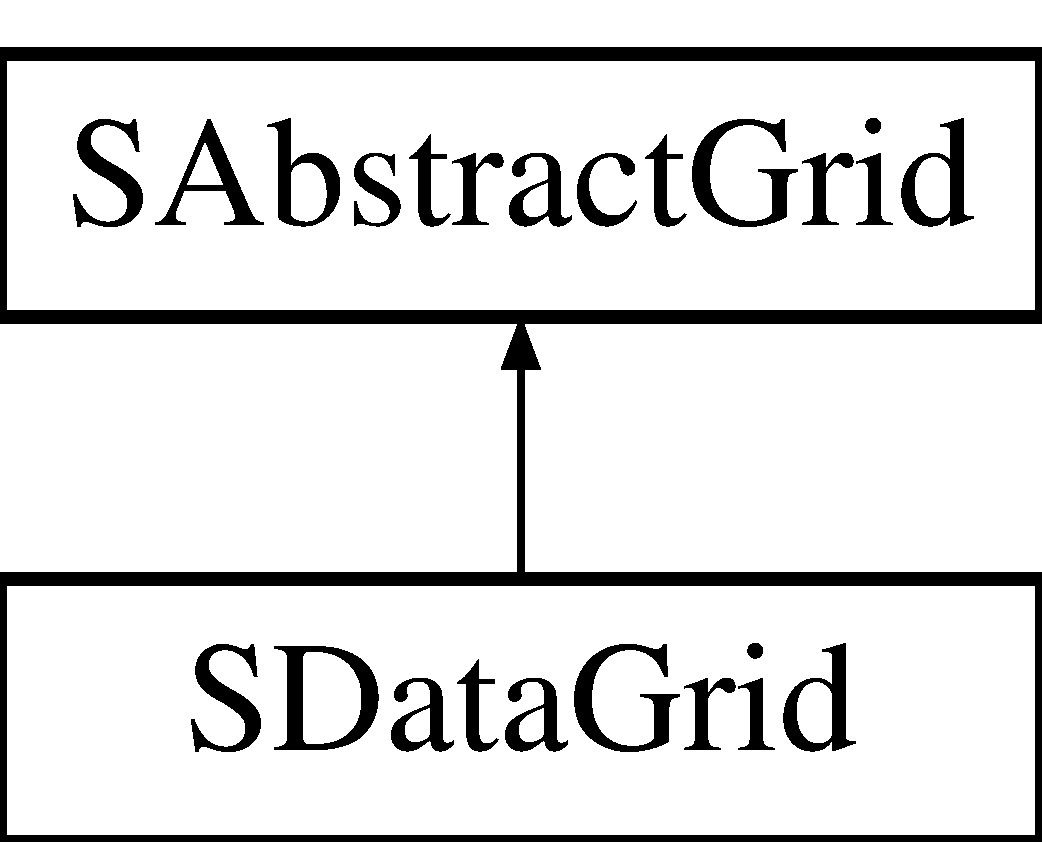
\includegraphics[height=2cm]{classSDataGrid}
\end{center}
\end{figure}
\subsection*{Metody publiczne}
\begin{CompactItemize}
\item 
\hyperlink{classSDataGrid_741ea12ba0eec8c00fec30c8730f2192}{SDataGrid} ()
\item 
\hyperlink{classSDataGrid_51645b217b4c668e0e945cdbda1db3ec}{$\sim$SDataGrid} ()
\item 
\hypertarget{classSDataGrid_7f9dd63d74e36731875630a96ea8dd07}{
int \textbf{getValueAt} (int, int)}
\label{classSDataGrid_7f9dd63d74e36731875630a96ea8dd07}

\item 
\hypertarget{classSDataGrid_fb34906c27b14e12fed01747f5763e68}{
int \textbf{performZeroAt} (int, int)}
\label{classSDataGrid_fb34906c27b14e12fed01747f5763e68}

\item 
\hypertarget{classSDataGrid_efb7f5da116641e2be648a6c8ad87643}{
int \textbf{performSuccAt} (int, int)}
\label{classSDataGrid_efb7f5da116641e2be648a6c8ad87643}

\item 
\hypertarget{classSDataGrid_c0b8507ad56abd1cd084e7a0c2218347}{
int \textbf{performPredAt} (int, int)}
\label{classSDataGrid_c0b8507ad56abd1cd084e7a0c2218347}

\item 
\hypertarget{classSDataGrid_8b94af72ddf880b0297baf24ceb2395a}{
void \textbf{\_\-\_\-dev\_\-\_\-printConsole} (int, int)}
\label{classSDataGrid_8b94af72ddf880b0297baf24ceb2395a}

\item 
\hypertarget{classSDataGrid_8421b3a44bfa7f38fd99cd9b5338ecc1}{
int \textbf{\_\-\_\-dev\_\-\_\-transformCharToBinary} (char)}
\label{classSDataGrid_8421b3a44bfa7f38fd99cd9b5338ecc1}

\item 
\hypertarget{classSDataGrid_8b1d40667ed06f454071faeaaa802b66}{
char \textbf{\_\-\_\-dev\_\-\_\-transformBinaryToChar} (int)}
\label{classSDataGrid_8b1d40667ed06f454071faeaaa802b66}

\end{CompactItemize}
\subsection*{Metody chronione}
\begin{CompactItemize}
\item 
\hypertarget{classSDataGrid_5af888335764c1ba959b6ef964223b6d}{
void \textbf{constructGrid} ()}
\label{classSDataGrid_5af888335764c1ba959b6ef964223b6d}

\item 
\hypertarget{classSDataGrid_c9c0ef298fb96c56f9f9796720a41489}{
void \textbf{destructGrid} ()}
\label{classSDataGrid_c9c0ef298fb96c56f9f9796720a41489}

\item 
\hypertarget{classSDataGrid_df36584ac2e2d38eda1bd06ad8fad355}{
void \textbf{zeroGrid} ()}
\label{classSDataGrid_df36584ac2e2d38eda1bd06ad8fad355}

\end{CompactItemize}
\subsection*{Atrybuty chronione}
\begin{CompactItemize}
\item 
\hypertarget{classSDataGrid_6401d181afc8b06f75fcec860b02e9cb}{
int $\ast$$\ast$ \textbf{data\_\-grid}}
\label{classSDataGrid_6401d181afc8b06f75fcec860b02e9cb}

\end{CompactItemize}


\subsection{Opis szczegółowy}
siatka danych 

Klasa ta umożliwia reprezentację obrazu danych w pamięci komputera. 

\subsection{Dokumentacja konstruktora i destruktora}
\hypertarget{classSDataGrid_741ea12ba0eec8c00fec30c8730f2192}{
\index{SDataGrid@{SDataGrid}!SDataGrid@{SDataGrid}}
\index{SDataGrid@{SDataGrid}!SDataGrid@{SDataGrid}}
\subsubsection[{SDataGrid}]{\setlength{\rightskip}{0pt plus 5cm}SDataGrid::SDataGrid ()}}
\label{classSDataGrid_741ea12ba0eec8c00fec30c8730f2192}


Konstruktor siatki danych. \hypertarget{classSDataGrid_51645b217b4c668e0e945cdbda1db3ec}{
\index{SDataGrid@{SDataGrid}!$\sim$SDataGrid@{$\sim$SDataGrid}}
\index{$\sim$SDataGrid@{$\sim$SDataGrid}!SDataGrid@{SDataGrid}}
\subsubsection[{$\sim$SDataGrid}]{\setlength{\rightskip}{0pt plus 5cm}SDataGrid::$\sim$SDataGrid ()}}
\label{classSDataGrid_51645b217b4c668e0e945cdbda1db3ec}


Destruktor siatki danych. 

Dokumentacja dla tej klasy została wygenerowana z plików:\begin{CompactItemize}
\item 
src/core/\hyperlink{sdatagrid_8h}{sdatagrid.h}\item 
src/core/\hyperlink{sdatagrid_8cpp}{sdatagrid.cpp}\end{CompactItemize}

\hypertarget{classSDataImagePointer}{
\section{Dokumentacja klasy SDataImagePointer}
\label{classSDataImagePointer}\index{SDataImagePointer@{SDataImagePointer}}
}
głowica maszyny obsługująca obraz danych  


{\tt \#include $<$sdataimagepointer.h$>$}

Diagram dziedziczenia dla SDataImagePointer:\begin{figure}[H]
\begin{center}
\leavevmode
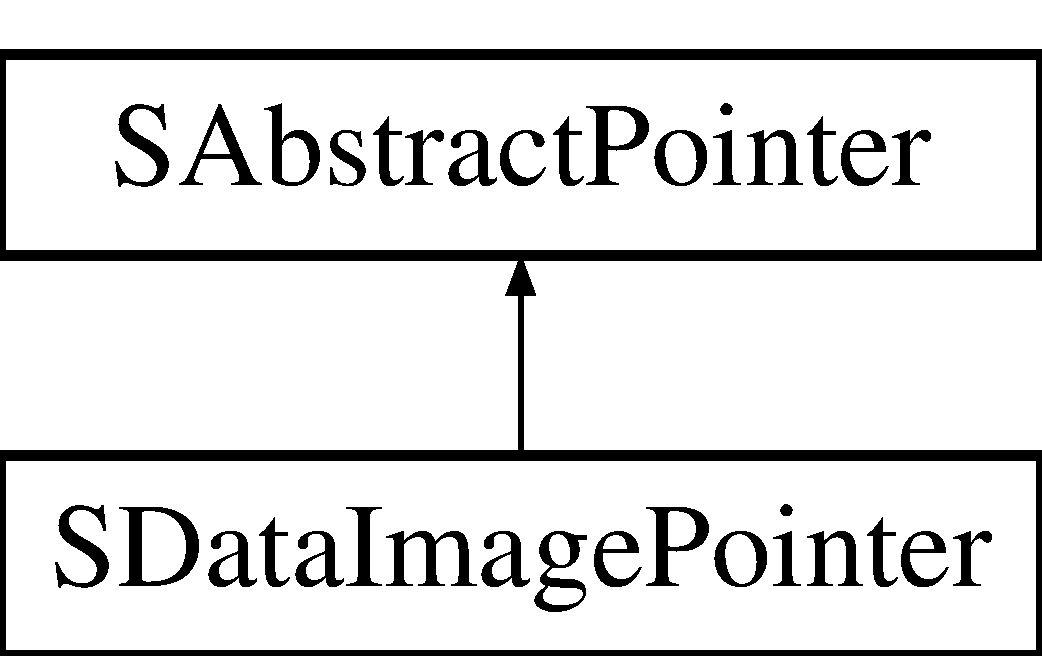
\includegraphics[height=2cm]{classSDataImagePointer}
\end{center}
\end{figure}
\subsection*{Metody publiczne}
\begin{CompactItemize}
\item 
\hyperlink{classSDataImagePointer_2ffb42e886f442004cd21617a6ea034d}{SDataImagePointer} ()
\item 
\hyperlink{classSDataImagePointer_8f96c4dc8dc25e0ff5cccb2e693ffcc8}{$\sim$SDataImagePointer} ()
\item 
int \hyperlink{classSDataImagePointer_87bb92d4bb0336b4723c64d03df9987c}{moveLeft} ()
\begin{CompactList}\small\item\em przesuwa głowicę maszyny danych w lewo \item\end{CompactList}\item 
int \hyperlink{classSDataImagePointer_9cc51881224c9e157e96d5e36189e54a}{moveRight} ()
\begin{CompactList}\small\item\em przesuwa głowicę maszyny danych w prawo \item\end{CompactList}\item 
\hypertarget{classSDataImagePointer_0cdd7239181d6f12bf6df551defaa769}{
int \textbf{increaseCellValue} ()}
\label{classSDataImagePointer_0cdd7239181d6f12bf6df551defaa769}

\item 
\hypertarget{classSDataImagePointer_0461b9855715a2d296e19865517f7f36}{
int \textbf{decreaseCellValue} ()}
\label{classSDataImagePointer_0461b9855715a2d296e19865517f7f36}

\item 
\hypertarget{classSDataImagePointer_ee071148492c43291fd01fd035f6398a}{
int \textbf{zeroCellValue} ()}
\label{classSDataImagePointer_ee071148492c43291fd01fd035f6398a}

\end{CompactItemize}


\subsection{Opis szczegółowy}
głowica maszyny obsługująca obraz danych 

Obiekt klasy \hyperlink{classSDataImagePointer}{SDataImagePointer} jest swoistym wskaźnikiem na daną komórkę obrazu danych. Maszyna danych (\hyperlink{classSDataMachine}{SDataMachine}) wykorzystuje głowicę, by dzięki niej odczytywać wartości z obrazu danych (SDataImage) oraz by na tym obrazie zapisywać nowe wartości. 

\subsection{Dokumentacja konstruktora i destruktora}
\hypertarget{classSDataImagePointer_2ffb42e886f442004cd21617a6ea034d}{
\index{SDataImagePointer@{SDataImagePointer}!SDataImagePointer@{SDataImagePointer}}
\index{SDataImagePointer@{SDataImagePointer}!SDataImagePointer@{SDataImagePointer}}
\subsubsection[{SDataImagePointer}]{\setlength{\rightskip}{0pt plus 5cm}SDataImagePointer::SDataImagePointer ()}}
\label{classSDataImagePointer_2ffb42e886f442004cd21617a6ea034d}


Konstruktor głowicy obrazu danych. Nie robi nic szczególnego. \hypertarget{classSDataImagePointer_8f96c4dc8dc25e0ff5cccb2e693ffcc8}{
\index{SDataImagePointer@{SDataImagePointer}!$\sim$SDataImagePointer@{$\sim$SDataImagePointer}}
\index{$\sim$SDataImagePointer@{$\sim$SDataImagePointer}!SDataImagePointer@{SDataImagePointer}}
\subsubsection[{$\sim$SDataImagePointer}]{\setlength{\rightskip}{0pt plus 5cm}SDataImagePointer::$\sim$SDataImagePointer ()}}
\label{classSDataImagePointer_8f96c4dc8dc25e0ff5cccb2e693ffcc8}


Destruktor głowicy obrazu danych. Nie robi nic szczególnego. 

\subsection{Dokumentacja funkcji składowych}
\hypertarget{classSDataImagePointer_87bb92d4bb0336b4723c64d03df9987c}{
\index{SDataImagePointer@{SDataImagePointer}!moveLeft@{moveLeft}}
\index{moveLeft@{moveLeft}!SDataImagePointer@{SDataImagePointer}}
\subsubsection[{moveLeft}]{\setlength{\rightskip}{0pt plus 5cm}int SDataImagePointer::moveLeft ()}}
\label{classSDataImagePointer_87bb92d4bb0336b4723c64d03df9987c}


przesuwa głowicę maszyny danych w lewo 

Najpierw ustalony jest nowy kierunek ruchu (SDirections) - w lewo, następnie głowica przesuwana jest o jedno pole (w ustalonym kierunku). Efektem przesunięcia głowicy jest zmiana jej współrzędnych względem obrazu danych. \begin{Desc}
\item[Zwraca:]? \end{Desc}
\hypertarget{classSDataImagePointer_9cc51881224c9e157e96d5e36189e54a}{
\index{SDataImagePointer@{SDataImagePointer}!moveRight@{moveRight}}
\index{moveRight@{moveRight}!SDataImagePointer@{SDataImagePointer}}
\subsubsection[{moveRight}]{\setlength{\rightskip}{0pt plus 5cm}int SDataImagePointer::moveRight ()}}
\label{classSDataImagePointer_9cc51881224c9e157e96d5e36189e54a}


przesuwa głowicę maszyny danych w prawo 

Najpierw ustalony jest nowy kierunek ruchu (SDirections) - w prawo, następnie głowica przesuwana jest o jedno pole (w ustalonym kierunku). Efektem przesunięcia głowicy jest zmiana jej współrzędnych względem obrazu danych. \begin{Desc}
\item[Zwraca:]? \end{Desc}


Dokumentacja dla tej klasy została wygenerowana z plików:\begin{CompactItemize}
\item 
src/core/\hyperlink{sdataimagepointer_8h}{sdataimagepointer.h}\item 
src/core/\hyperlink{sdataimagepointer_8cpp}{sdataimagepointer.cpp}\end{CompactItemize}

\hypertarget{classSDataMachine}{
\section{Dokumentacja klasy SDataMachine}
\label{classSDataMachine}\index{SDataMachine@{SDataMachine}}
}
maszyna danych, obsługująca obraz danych  


{\tt \#include $<$sdatamachine.h$>$}

Diagram dziedziczenia dla SDataMachine:\begin{figure}[H]
\begin{center}
\leavevmode
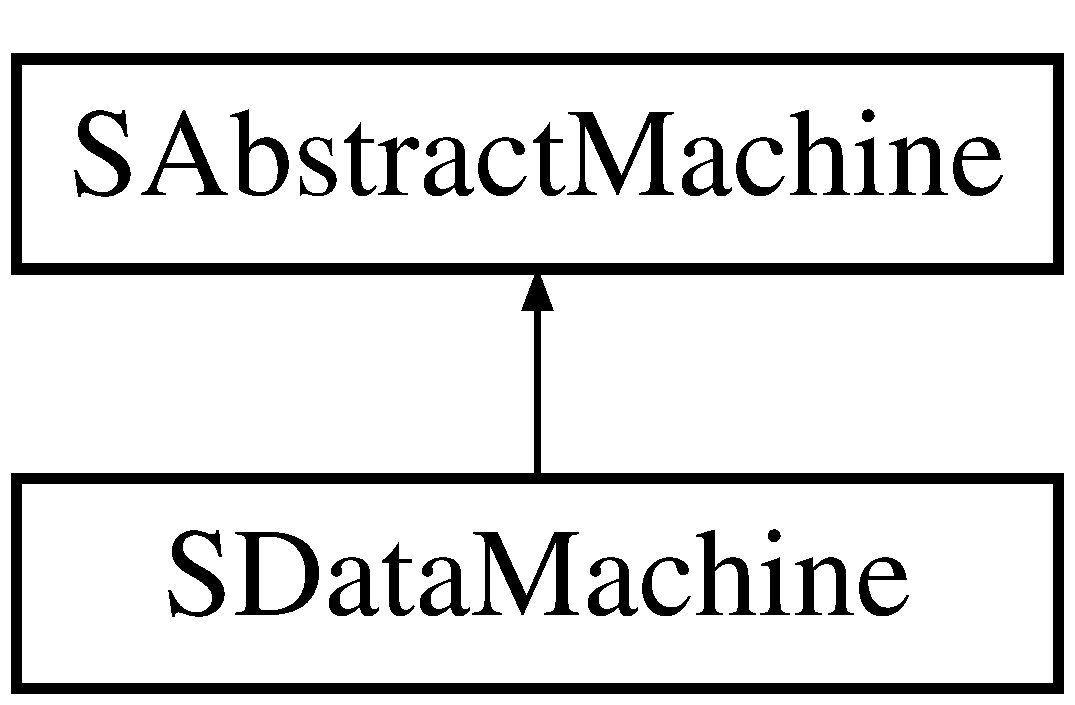
\includegraphics[height=2cm]{classSDataMachine}
\end{center}
\end{figure}
\subsection*{Metody publiczne}
\begin{CompactItemize}
\item 
\hyperlink{classSDataMachine_3d894df00bd2283c717a827e27138812}{SDataMachine} ()
\begin{CompactList}\small\item\em konstruktor \item\end{CompactList}\item 
\hyperlink{classSDataMachine_59bc85b25930729cbe3046e81f49f909}{$\sim$SDataMachine} ()
\begin{CompactList}\small\item\em destruktor \item\end{CompactList}\item 
void \hyperlink{classSDataMachine_38cc38f27606be24fc609d461d25ae2f}{setVerbosity} (bool)
\item 
bool \hyperlink{classSDataMachine_10eb8f56cf6235455a26c5c673b8fe15}{pushPointer} ()
\item 
void \hyperlink{classSDataMachine_b863ea9a42568d7555cc146ded9f2d88}{clearData} ()
\item 
int \hyperlink{classSDataMachine_3a191be9cab718274d6bd75e01cc2a26}{getPointedValue} ()
\item 
void \hyperlink{classSDataMachine_5b46d50c18bec1bcfd5232bec3875fd5}{executeTurnLeft} ()
\item 
void \hyperlink{classSDataMachine_fb6f52c7f14afa51eed848f354d57924}{executeTurnRight} ()
\item 
void \hyperlink{classSDataMachine_27c3e6dfe9ac45f9d5eed7c97f96abd8}{executeZero} ()
\item 
void \hyperlink{classSDataMachine_85832e07e2fb8ae32160fe0c95a487d2}{executeSucc} ()
\item 
void \hyperlink{classSDataMachine_87cfad868b3ea0a0e60f776ad3773678}{executePred} ()
\item 
\hypertarget{classSDataMachine_9680a908e0343de539ffd7a83d17dd11}{
void \textbf{\_\-\_\-dev\_\-\_\-initGrid} ()}
\label{classSDataMachine_9680a908e0343de539ffd7a83d17dd11}

\item 
\hypertarget{classSDataMachine_66c35c3c879c06903f306825ccaade7f}{
void \textbf{\_\-\_\-dev\_\-\_\-destroyGrid} ()}
\label{classSDataMachine_66c35c3c879c06903f306825ccaade7f}

\item 
\hypertarget{classSDataMachine_da92c5d20a64279ff191059705c3070f}{
void \textbf{\_\-\_\-dev\_\-\_\-printConsole} ()}
\label{classSDataMachine_da92c5d20a64279ff191059705c3070f}

\item 
\hypertarget{classSDataMachine_3d2383297382e73c4f61f7fc231c34b7}{
void \textbf{\_\-\_\-dev\_\-\_\-printPointer} ()}
\label{classSDataMachine_3d2383297382e73c4f61f7fc231c34b7}

\item 
\hypertarget{classSDataMachine_ec760b755d01ea8c9ef3d37aa8f749d2}{
void \textbf{\_\-\_\-dev\_\-\_\-printGrid} ()}
\label{classSDataMachine_ec760b755d01ea8c9ef3d37aa8f749d2}

\end{CompactItemize}


\subsection{Opis szczegółowy}
maszyna danych, obsługująca obraz danych 

Obiekt klasy \hyperlink{classSDataMachine}{SDataMachine} to tzw. \char`\"{}maszyna danych\char`\"{} która obsługuje dane programu wykonywanego przez Wirtualną Maszynę Salvadora. Maszyna ta posiada swój log (dziennik wszystkich wykonywanych operacji) w obiekcie klasy SDataStats oraz posiada sam obraz danych, będący graficzną reprezentacją danych wykonywanego programu. 

\subsection{Dokumentacja konstruktora i destruktora}
\hypertarget{classSDataMachine_3d894df00bd2283c717a827e27138812}{
\index{SDataMachine@{SDataMachine}!SDataMachine@{SDataMachine}}
\index{SDataMachine@{SDataMachine}!SDataMachine@{SDataMachine}}
\subsubsection[{SDataMachine}]{\setlength{\rightskip}{0pt plus 5cm}SDataMachine::SDataMachine ()}}
\label{classSDataMachine_3d894df00bd2283c717a827e27138812}


konstruktor 

Tworzy 3 obiekty, do których ma zapisane referencje:\begin{itemize}
\item log operacji maszyny danych (SDataStats)\item obraz danych (SDataImage)\item głowica maszyny danych (\hyperlink{classSDataImagePointer}{SDataImagePointer}) Maszyna danych w trakcie swojego działania będzie z nich cały czas korzystać \end{itemize}
\hypertarget{classSDataMachine_59bc85b25930729cbe3046e81f49f909}{
\index{SDataMachine@{SDataMachine}!$\sim$SDataMachine@{$\sim$SDataMachine}}
\index{$\sim$SDataMachine@{$\sim$SDataMachine}!SDataMachine@{SDataMachine}}
\subsubsection[{$\sim$SDataMachine}]{\setlength{\rightskip}{0pt plus 5cm}SDataMachine::$\sim$SDataMachine ()}}
\label{classSDataMachine_59bc85b25930729cbe3046e81f49f909}


destruktor 

Niszczy 3 obiekty, niezbędne do działania maszyny:\begin{itemize}
\item log operacji maszyny danych (SDataStats)\item obraz danych (SDataImage)\item głowica maszyny danych (\hyperlink{classSDataImagePointer}{SDataImagePointer}) \end{itemize}


\subsection{Dokumentacja funkcji składowych}
\hypertarget{classSDataMachine_b863ea9a42568d7555cc146ded9f2d88}{
\index{SDataMachine@{SDataMachine}!clearData@{clearData}}
\index{clearData@{clearData}!SDataMachine@{SDataMachine}}
\subsubsection[{clearData}]{\setlength{\rightskip}{0pt plus 5cm}void SDataMachine::clearData ()}}
\label{classSDataMachine_b863ea9a42568d7555cc146ded9f2d88}


Czyści dane przechowywane przez maszynę danych. \hypertarget{classSDataMachine_87cfad868b3ea0a0e60f776ad3773678}{
\index{SDataMachine@{SDataMachine}!executePred@{executePred}}
\index{executePred@{executePred}!SDataMachine@{SDataMachine}}
\subsubsection[{executePred}]{\setlength{\rightskip}{0pt plus 5cm}void SDataMachine::executePred ()}}
\label{classSDataMachine_87cfad868b3ea0a0e60f776ad3773678}


Wykonuje instrukcję Salvadora ZMNIEJSZ. \hypertarget{classSDataMachine_85832e07e2fb8ae32160fe0c95a487d2}{
\index{SDataMachine@{SDataMachine}!executeSucc@{executeSucc}}
\index{executeSucc@{executeSucc}!SDataMachine@{SDataMachine}}
\subsubsection[{executeSucc}]{\setlength{\rightskip}{0pt plus 5cm}void SDataMachine::executeSucc ()}}
\label{classSDataMachine_85832e07e2fb8ae32160fe0c95a487d2}


Wykonuje instrukcję Salvadora ZWIĘKSZ. \hypertarget{classSDataMachine_5b46d50c18bec1bcfd5232bec3875fd5}{
\index{SDataMachine@{SDataMachine}!executeTurnLeft@{executeTurnLeft}}
\index{executeTurnLeft@{executeTurnLeft}!SDataMachine@{SDataMachine}}
\subsubsection[{executeTurnLeft}]{\setlength{\rightskip}{0pt plus 5cm}void SDataMachine::executeTurnLeft ()}}
\label{classSDataMachine_5b46d50c18bec1bcfd5232bec3875fd5}


Wykonuje instrukcję Salvadora PRZESUŃ GŁOWICĘ DANYCH W LEWO. \hypertarget{classSDataMachine_fb6f52c7f14afa51eed848f354d57924}{
\index{SDataMachine@{SDataMachine}!executeTurnRight@{executeTurnRight}}
\index{executeTurnRight@{executeTurnRight}!SDataMachine@{SDataMachine}}
\subsubsection[{executeTurnRight}]{\setlength{\rightskip}{0pt plus 5cm}void SDataMachine::executeTurnRight ()}}
\label{classSDataMachine_fb6f52c7f14afa51eed848f354d57924}


Wykonuje instrukcję Salvadora PRZESUŃ GŁOWICĘ DANYCH W PRAWO. \hypertarget{classSDataMachine_27c3e6dfe9ac45f9d5eed7c97f96abd8}{
\index{SDataMachine@{SDataMachine}!executeZero@{executeZero}}
\index{executeZero@{executeZero}!SDataMachine@{SDataMachine}}
\subsubsection[{executeZero}]{\setlength{\rightskip}{0pt plus 5cm}void SDataMachine::executeZero ()}}
\label{classSDataMachine_27c3e6dfe9ac45f9d5eed7c97f96abd8}


Wykonuje instrukcję Salvadora ZERUJ. \hypertarget{classSDataMachine_3a191be9cab718274d6bd75e01cc2a26}{
\index{SDataMachine@{SDataMachine}!getPointedValue@{getPointedValue}}
\index{getPointedValue@{getPointedValue}!SDataMachine@{SDataMachine}}
\subsubsection[{getPointedValue}]{\setlength{\rightskip}{0pt plus 5cm}int SDataMachine::getPointedValue ()}}
\label{classSDataMachine_3a191be9cab718274d6bd75e01cc2a26}


Zwraca wartość wskazywaną przez głowicę danych na obrazie danych. \begin{Desc}
\item[Zwraca:]wartość wskazywana przez głowicę \end{Desc}
\hypertarget{classSDataMachine_10eb8f56cf6235455a26c5c673b8fe15}{
\index{SDataMachine@{SDataMachine}!pushPointer@{pushPointer}}
\index{pushPointer@{pushPointer}!SDataMachine@{SDataMachine}}
\subsubsection[{pushPointer}]{\setlength{\rightskip}{0pt plus 5cm}bool SDataMachine::pushPointer ()\hspace{0.3cm}{\tt  \mbox{[}virtual\mbox{]}}}}
\label{classSDataMachine_10eb8f56cf6235455a26c5c673b8fe15}


Przesuwa głowicę danych o jedną komórkę w bieżącym kierunku. \begin{Desc}
\item[Zwraca:]czy się udało; w przypadku maszyny danych zawsze się udaje \end{Desc}


Implementuje \hyperlink{classSAbstractMachine_72a47b72416e0d2f24fcf36415d37404}{SAbstractMachine}.\hypertarget{classSDataMachine_38cc38f27606be24fc609d461d25ae2f}{
\index{SDataMachine@{SDataMachine}!setVerbosity@{setVerbosity}}
\index{setVerbosity@{setVerbosity}!SDataMachine@{SDataMachine}}
\subsubsection[{setVerbosity}]{\setlength{\rightskip}{0pt plus 5cm}void SDataMachine::setVerbosity (bool {\em verbosity})}}
\label{classSDataMachine_38cc38f27606be24fc609d461d25ae2f}


Ustala tryb gadatliwy. \begin{Desc}
\item[Parametry:]
\begin{description}
\item[{\em verbosity}]tryb gadatliwy \end{description}
\end{Desc}


Dokumentacja dla tej klasy została wygenerowana z plików:\begin{CompactItemize}
\item 
src/core/\hyperlink{sdatamachine_8h}{sdatamachine.h}\item 
src/core/\hyperlink{sdatamachine_8cpp}{sdatamachine.cpp}\end{CompactItemize}

\hypertarget{classSVirtualMachine}{
\section{Dokumentacja klasy SVirtualMachine}
\label{classSVirtualMachine}\index{SVirtualMachine@{SVirtualMachine}}
}
wirtualna maszyna Salvadora - najbardziej \char`\"{}zewnętrzna\char`\"{} klasa całego projektu  


{\tt \#include $<$svirtualmachine.h$>$}

\subsection*{Metody publiczne}
\begin{CompactItemize}
\item 
\hypertarget{classSVirtualMachine_020a4e9202a688dffed1e0d8951f9164}{
\textbf{SVirtualMachine} (std::string, \hyperlink{senums_8h_1a2ae45552936d27425f99e1c187b043}{SCodeTypes})}
\label{classSVirtualMachine_020a4e9202a688dffed1e0d8951f9164}

\item 
\hypertarget{classSVirtualMachine_09f1f983396791f84947f80097351862}{
bool \textbf{isRunning} ()}
\label{classSVirtualMachine_09f1f983396791f84947f80097351862}

\item 
\hypertarget{classSVirtualMachine_86dfbb99cbccd36729253cf34835c805}{
bool \textbf{isReady} ()}
\label{classSVirtualMachine_86dfbb99cbccd36729253cf34835c805}

\item 
\hypertarget{classSVirtualMachine_3c530338eaccb6bc585ba689ace469a7}{
void \textbf{startMachine} ()}
\label{classSVirtualMachine_3c530338eaccb6bc585ba689ace469a7}

\item 
\hypertarget{classSVirtualMachine_6b2dedbf7e71aeb57c89ada07141a2d1}{
void \textbf{restartMachine} ()}
\label{classSVirtualMachine_6b2dedbf7e71aeb57c89ada07141a2d1}

\item 
\hypertarget{classSVirtualMachine_47097e43ad093ef4900df2d888043da6}{
void \textbf{stopMachine} ()}
\label{classSVirtualMachine_47097e43ad093ef4900df2d888043da6}

\item 
\hypertarget{classSVirtualMachine_85f2b4a688a077283010a11145289110}{
void \textbf{clean} ()}
\label{classSVirtualMachine_85f2b4a688a077283010a11145289110}

\item 
void \hyperlink{classSVirtualMachine_f3874f10dac15f27b23dc4b976271413}{executeAllInstr} ()
\item 
\hypertarget{classSVirtualMachine_200c4aae4eedf52ba7a3754295505186}{
void \textbf{executeInstr} ()}
\label{classSVirtualMachine_200c4aae4eedf52ba7a3754295505186}

\item 
\hypertarget{classSVirtualMachine_2a2a23e279ef7df99fbcdd798a5385cf}{
bool \textbf{revokeInstr} ()}
\label{classSVirtualMachine_2a2a23e279ef7df99fbcdd798a5385cf}

\item 
\hypertarget{classSVirtualMachine_c8d0c7a837c157b0a1efaf80ffeee486}{
bool \textbf{goBack} (int)}
\label{classSVirtualMachine_c8d0c7a837c157b0a1efaf80ffeee486}

\item 
\hypertarget{classSVirtualMachine_f8e1ef67bff80a4ce0aa7afc741a1a93}{
std::string \textbf{\_\-\_\-dev\_\-\_\-transformBinaryStateToString} (\hyperlink{senums_8h_c31b206c0c7cd52b9a0b18204f373c7e}{SMachineStates})}
\label{classSVirtualMachine_f8e1ef67bff80a4ce0aa7afc741a1a93}

\item 
\hypertarget{classSVirtualMachine_21b1ac24c7018fd084a553a66f5827ea}{
void \textbf{\_\-\_\-dev\_\-\_\-printConsole} ()}
\label{classSVirtualMachine_21b1ac24c7018fd084a553a66f5827ea}

\item 
\hypertarget{classSVirtualMachine_cf39eaf295cf709c43b8754aed84286f}{
void \textbf{\_\-\_\-dev\_\-\_\-destroyGrid} ()}
\label{classSVirtualMachine_cf39eaf295cf709c43b8754aed84286f}

\item 
void \hyperlink{classSVirtualMachine_d07f353daaf626f5efeb8bd34818db75}{\_\-\_\-dev\_\-\_\-runProgram} ()
\begin{CompactList}\small\item\em symulacja działania wirtualnej maszyny \item\end{CompactList}\end{CompactItemize}


\subsection{Opis szczegółowy}
wirtualna maszyna Salvadora - najbardziej \char`\"{}zewnętrzna\char`\"{} klasa całego projektu 

Wirtualna maszyna Salvadora jest czymś w stylu opakowania, które kryje w sobie wszystkie mechanizmy interpretera. Do działania używa dwóch pozostałych maszyn: maszyny kodu (\hyperlink{classSCodeMachine}{SCodeMachine}) oraz maszyny danych (\hyperlink{classSDataMachine}{SDataMachine}); zarządza czasem życia obu z nich.

Działanie wirtualnej maszyny Salvadora:

Maszyna musi być ustawiona w stanie 'ready' (SMachineStates, jest to możliwe przy pomocy metody XXX lub od razu po wywołaniu konstruktora). Metoda YYY przełącza wirtualną maszynę w stan działania (SMachineStates, 'running'). Następnie przy pomocy metody ZZZ można zlecać maszynie wykonanie pojedynczej instrukcji intepretera.

Wykonanie pojedynczej instrukcji:

\begin{itemize}
\item wirtualna maszyna zleca maszynie kodu (\hyperlink{classSCodeMachine}{SCodeMachine}) sprawdzenie jaka instrukcja (SCodeInstructions, SDataInstructions) ma zostać wykonana.\item maszyna kodu (\hyperlink{classSCodeMachine}{SCodeMachine}) zwraca maszynie wirtualnej informację o instrukcji\item w zależności od rodzaju instrukcji, maszyna wirtualna zleca jej wykonanie maszynie kodu (\hyperlink{classSCodeMachine}{SCodeMachine}, SCodeInstructions) lub maszynie danych (\hyperlink{classSDataMachine}{SDataMachine}, SDataInstructions)\item maszyna wykonująca instrukcję, zapisuje ją w swoim logu (SCodeStats, SDataStats)\item maszyna kodu (\hyperlink{classSCodeMachine}{SCodeMachine}) przesuwa swoją głowicę (\hyperlink{classSCodeImagePointer}{SCodeImagePointer}) w dotychczasowym kierunku \end{itemize}


\subsection{Dokumentacja funkcji składowych}
\hypertarget{classSVirtualMachine_d07f353daaf626f5efeb8bd34818db75}{
\index{SVirtualMachine@{SVirtualMachine}!\_\-\_\-dev\_\-\_\-runProgram@{\_\-\_\-dev\_\-\_\-runProgram}}
\index{\_\-\_\-dev\_\-\_\-runProgram@{\_\-\_\-dev\_\-\_\-runProgram}!SVirtualMachine@{SVirtualMachine}}
\subsubsection[{\_\-\_\-dev\_\-\_\-runProgram}]{\setlength{\rightskip}{0pt plus 5cm}void SVirtualMachine::\_\-\_\-dev\_\-\_\-runProgram ()}}
\label{classSVirtualMachine_d07f353daaf626f5efeb8bd34818db75}


symulacja działania wirtualnej maszyny 

DEVELOPMENT

Konsolowo symyluje przebieg działania maszyny. Najpierw wyświetla dane obu maszyn, następnie po każdym kroku wyświetla wynik na konsoli. Przy każdym kroku użytkownik ma możliwość zastopowania działania maszyny, wpisując frazę \char`\"{}no\char`\"{}. Metoda kończy działanie, kiedy maszyna skończy swoje działanie. \hypertarget{classSVirtualMachine_f3874f10dac15f27b23dc4b976271413}{
\index{SVirtualMachine@{SVirtualMachine}!executeAllInstr@{executeAllInstr}}
\index{executeAllInstr@{executeAllInstr}!SVirtualMachine@{SVirtualMachine}}
\subsubsection[{executeAllInstr}]{\setlength{\rightskip}{0pt plus 5cm}void SVirtualMachine::executeAllInstr ()}}
\label{classSVirtualMachine_f3874f10dac15f27b23dc4b976271413}


Wykonuje wszystkie instrukcje 

Dokumentacja dla tej klasy została wygenerowana z plików:\begin{CompactItemize}
\item 
src/core/\hyperlink{svirtualmachine_8h}{svirtualmachine.h}\item 
src/core/\hyperlink{svirtualmachine_8cpp}{svirtualmachine.cpp}\end{CompactItemize}

\chapter{Dokumentacja plików}
\hypertarget{sabstractgrid_8cpp}{
\section{Dokumentacja pliku src/core/sabstractgrid.cpp}
\label{sabstractgrid_8cpp}\index{src/core/sabstractgrid.cpp@{src/core/sabstractgrid.cpp}}
}
Plik z kodem źródłowym klasy \hyperlink{classSAbstractGrid}{SAbstractGrid}.  


{\tt \#include \char`\"{}sabstractgrid.h\char`\"{}}\par
{\tt \#include \char`\"{}../debug.h\char`\"{}}\par
{\tt \#include \char`\"{}senums.h\char`\"{}}\par
{\tt \#include $<$string$>$}\par
{\tt \#include $<$fstream$>$}\par
{\tt \#include $<$iostream$>$}\par


\subsection{Opis szczegółowy}
Plik z kodem źródłowym klasy \hyperlink{classSAbstractGrid}{SAbstractGrid}. 

Plik zawiera kod źródłowy klasy \hyperlink{classSAbstractGrid}{SAbstractGrid}. 
\hypertarget{sabstractgrid_8h}{
\section{Dokumentacja pliku src/core/sabstractgrid.h}
\label{sabstractgrid_8h}\index{src/core/sabstractgrid.h@{src/core/sabstractgrid.h}}
}
Plik nagłówkowy klasy \hyperlink{classSAbstractGrid}{SAbstractGrid}.  


{\tt \#include \char`\"{}senums.h\char`\"{}}\par
{\tt \#include $<$string$>$}\par
\subsection*{Komponenty}
\begin{CompactItemize}
\item 
class \hyperlink{classSAbstractGrid}{SAbstractGrid}
\begin{CompactList}\small\item\em Sbstrakcyjna siatka. \item\end{CompactList}\end{CompactItemize}


\subsection{Opis szczegółowy}
Plik nagłówkowy klasy \hyperlink{classSAbstractGrid}{SAbstractGrid}. 

Plik zawiera definicję klasy \hyperlink{classSAbstractGrid}{SAbstractGrid}. Obiekty tej klasy reprezentują abstrakcyjną siatkę wykorzystywaną przez programy języka Salvador 
\hypertarget{sabstractmachine_8cpp}{
\section{Dokumentacja pliku src/core/sabstractmachine.cpp}
\label{sabstractmachine_8cpp}\index{src/core/sabstractmachine.cpp@{src/core/sabstractmachine.cpp}}
}
Plik z kodem źródłowym klasy \hyperlink{classSAbstractMachine}{SAbstractMachine}.  


{\tt \#include \char`\"{}sabstractmachine.h\char`\"{}}\par
{\tt \#include \char`\"{}../debug.h\char`\"{}}\par
{\tt \#include \char`\"{}senums.h\char`\"{}}\par
{\tt \#include \char`\"{}sabstractgrid.h\char`\"{}}\par
{\tt \#include $<$string$>$}\par
{\tt \#include $<$iostream$>$}\par


\subsection{Opis szczegółowy}
Plik z kodem źródłowym klasy \hyperlink{classSAbstractMachine}{SAbstractMachine}. 

Plik zawiera kod źródłowy klasy \hyperlink{classSAbstractMachine}{SAbstractMachine}. 
\hypertarget{sabstractmachine_8h}{
\section{Dokumentacja pliku src/core/sabstractmachine.h}
\label{sabstractmachine_8h}\index{src/core/sabstractmachine.h@{src/core/sabstractmachine.h}}
}
plik nagłówkowy klasy SAbstractMachine 

{\tt \#include \char`\"{}senums.h\char`\"{}}\par
{\tt \#include \char`\"{}sabstractpointer.h\char`\"{}}\par
{\tt \#include $<$string$>$}\par
\subsection*{Komponenty}
\begin{CompactItemize}
\item 
class \textbf{SAbstractMachine}
\end{CompactItemize}


\subsection{Opis szczegółowy}
plik nagłówkowy klasy SAbstractMachine 

Plik zawiera definicję klasy SAbstractMachine. Ma ona zdefiniowane podstawowe operacje na maszynach, dziedziczą po niej dwie najważniejsze klasy projektu: \hyperlink{classSDataMachine}{SDataMachine} i SCodeMachine. 
\hypertarget{sabstractpointer_8cpp}{
\section{Dokumentacja pliku src/core/sabstractpointer.cpp}
\label{sabstractpointer_8cpp}\index{src/core/sabstractpointer.cpp@{src/core/sabstractpointer.cpp}}
}
Plik z kodem źródłowym klasy \hyperlink{classSAbstractPointer}{SAbstractPointer}.  


{\tt \#include \char`\"{}sabstractpointer.h\char`\"{}}\par
{\tt \#include \char`\"{}../debug.h\char`\"{}}\par
{\tt \#include \char`\"{}senums.h\char`\"{}}\par
{\tt \#include $<$iostream$>$}\par
{\tt \#include $<$fstream$>$}\par
{\tt \#include $<$string$>$}\par


\subsection{Opis szczegółowy}
Plik z kodem źródłowym klasy \hyperlink{classSAbstractPointer}{SAbstractPointer}. 

Plik zawiera kod źródłowy klasy \hyperlink{classSAbstractPointer}{SAbstractPointer}. 
\hypertarget{sabstractpointer_8h}{
\section{Dokumentacja pliku src/core/sabstractpointer.h}
\label{sabstractpointer_8h}\index{src/core/sabstractpointer.h@{src/core/sabstractpointer.h}}
}
plik nagłówkowy klasy \hyperlink{classSAbstractPointer}{SAbstractPointer}  


{\tt \#include \char`\"{}senums.h\char`\"{}}\par
{\tt \#include $<$string$>$}\par
\subsection*{Komponenty}
\begin{CompactItemize}
\item 
class \hyperlink{classSAbstractPointer}{SAbstractPointer}
\begin{CompactList}\small\item\em abstrakcyjna głowica maszyn \item\end{CompactList}\end{CompactItemize}


\subsection{Opis szczegółowy}
plik nagłówkowy klasy \hyperlink{classSAbstractPointer}{SAbstractPointer} 

Plik zawiera definicję klasy \hyperlink{classSAbstractPointer}{SAbstractPointer}. Ma ona zdefiniowane podstawowe operacje na głowicach maszyn (maszyny kodu i maszyny danych) wykorzystywanych w Wirtualnej Maszynie Salvadora. 
\hypertarget{scodegrid_8cpp}{
\section{Dokumentacja pliku src/core/scodegrid.cpp}
\label{scodegrid_8cpp}\index{src/core/scodegrid.cpp@{src/core/scodegrid.cpp}}
}
Plik z kodem źródłowym klasy \hyperlink{classSCodeGrid}{SCodeGrid}.  


{\tt \#include \char`\"{}scodegrid.h\char`\"{}}\par
{\tt \#include \char`\"{}../debug.h\char`\"{}}\par
{\tt \#include \char`\"{}senums.h\char`\"{}}\par
{\tt \#include $<$string$>$}\par
{\tt \#include $<$fstream$>$}\par
{\tt \#include $<$iostream$>$}\par
{\tt \#include $<$QImage$>$}\par
{\tt \#include $<$QRgb$>$}\par


\subsection{Opis szczegółowy}
Plik z kodem źródłowym klasy \hyperlink{classSCodeGrid}{SCodeGrid}. 

Plik zawiera kod źródłowy klasy \hyperlink{classSCodeGrid}{SCodeGrid}. 
\hypertarget{scodegrid_8h}{
\section{Dokumentacja pliku src/core/scodegrid.h}
\label{scodegrid_8h}\index{src/core/scodegrid.h@{src/core/scodegrid.h}}
}
plik nagłówkowy klasy \hyperlink{classSCodeGrid}{SCodeGrid}  


{\tt \#include \char`\"{}senums.h\char`\"{}}\par
{\tt \#include \char`\"{}sabstractgrid.h\char`\"{}}\par
{\tt \#include $<$string$>$}\par
\subsection*{Komponenty}
\begin{CompactItemize}
\item 
class \hyperlink{classSCodeGrid}{SCodeGrid}
\begin{CompactList}\small\item\em siatka kodu \item\end{CompactList}\end{CompactItemize}


\subsection{Opis szczegółowy}
plik nagłówkowy klasy \hyperlink{classSCodeGrid}{SCodeGrid} 

Plik zawiera definicję klasy \hyperlink{classSCodeGrid}{SCodeGrid}. Obiekty tej klasy reprezentują siatkę kodu dowolnego programu w języku Salvador. 
\hypertarget{scodeimagepointer_8cpp}{
\section{Dokumentacja pliku src/core/scodeimagepointer.cpp}
\label{scodeimagepointer_8cpp}\index{src/core/scodeimagepointer.cpp@{src/core/scodeimagepointer.cpp}}
}
Plik z kodem źródłowym klasy \hyperlink{classSCodeImagePointer}{SCodeImagePointer}.  


{\tt \#include \char`\"{}scodeimagepointer.h\char`\"{}}\par
{\tt \#include \char`\"{}../debug.h\char`\"{}}\par
{\tt \#include \char`\"{}senums.h\char`\"{}}\par
{\tt \#include $<$string$>$}\par


\subsection{Opis szczegółowy}
Plik z kodem źródłowym klasy \hyperlink{classSCodeImagePointer}{SCodeImagePointer}. 

Plik zawiera kod źródłowy klasy \hyperlink{classSCodeImagePointer}{SCodeImagePointer}. 
\hypertarget{scodeimagepointer_8h}{
\section{Dokumentacja pliku src/core/scodeimagepointer.h}
\label{scodeimagepointer_8h}\index{src/core/scodeimagepointer.h@{src/core/scodeimagepointer.h}}
}
plik nagłówkowy klasy \hyperlink{classSCodeImagePointer}{SCodeImagePointer}  


{\tt \#include \char`\"{}senums.h\char`\"{}}\par
{\tt \#include \char`\"{}sabstractpointer.h\char`\"{}}\par
{\tt \#include $<$string$>$}\par
\subsection*{Komponenty}
\begin{CompactItemize}
\item 
class \hyperlink{classSCodeImagePointer}{SCodeImagePointer}
\begin{CompactList}\small\item\em głowica maszyny obsługująca obraz kodu \item\end{CompactList}\end{CompactItemize}


\subsection{Opis szczegółowy}
plik nagłówkowy klasy \hyperlink{classSCodeImagePointer}{SCodeImagePointer} 

Plik zawiera definicję klasy \hyperlink{classSCodeImagePointer}{SCodeImagePointer}. Obiekt tej klasy jest głowicą maszyny kodu. 
\hypertarget{scodemachine_8cpp}{
\section{Dokumentacja pliku src/core/scodemachine.cpp}
\label{scodemachine_8cpp}\index{src/core/scodemachine.cpp@{src/core/scodemachine.cpp}}
}
Plik z kodem źródłowym klasy \hyperlink{classSCodeMachine}{SCodeMachine}.  


{\tt \#include \char`\"{}scodemachine.h\char`\"{}}\par
{\tt \#include \char`\"{}../debug.h\char`\"{}}\par
{\tt \#include \char`\"{}senums.h\char`\"{}}\par
{\tt \#include \char`\"{}scodeimage.h\char`\"{}}\par
{\tt \#include \char`\"{}scodeimagepointer.h\char`\"{}}\par
{\tt \#include $<$string$>$}\par
{\tt \#include $<$iostream$>$}\par


\subsection{Opis szczegółowy}
Plik z kodem źródłowym klasy \hyperlink{classSCodeMachine}{SCodeMachine}. 

Plik zawiera kod źródłowy klasy \hyperlink{classSCodeMachine}{SCodeMachine}. 
\hypertarget{scodemachine_8h}{
\section{Dokumentacja pliku src/core/scodemachine.h}
\label{scodemachine_8h}\index{src/core/scodemachine.h@{src/core/scodemachine.h}}
}
plik nagłówkowy klasy \hyperlink{classSCodeMachine}{SCodeMachine}  


{\tt \#include \char`\"{}senums.h\char`\"{}}\par
{\tt \#include \char`\"{}sabstractmachine.h\char`\"{}}\par
{\tt \#include \char`\"{}scodeimagepointer.h\char`\"{}}\par
{\tt \#include \char`\"{}scodegrid.h\char`\"{}}\par
{\tt \#include $<$string$>$}\par
{\tt \#include $<$QImage$>$}\par
\subsection*{Komponenty}
\begin{CompactItemize}
\item 
class \hyperlink{classSCodeMachine}{SCodeMachine}
\begin{CompactList}\small\item\em maszyna danych, obsługująca obraz danych \item\end{CompactList}\end{CompactItemize}


\subsection{Opis szczegółowy}
plik nagłówkowy klasy \hyperlink{classSCodeMachine}{SCodeMachine} 

Plik zawiera definicję klasy \hyperlink{classSCodeMachine}{SCodeMachine}. Maszyna kodu to najważniejszy obiekt projektu Salvador, odpowiada on za działanie całości: wykonuje obliczenia, wymusza operacje innych obiektów (głowic, maszyny danych). 
\hypertarget{sdatagrid_8cpp}{
\section{Dokumentacja pliku src/core/sdatagrid.cpp}
\label{sdatagrid_8cpp}\index{src/core/sdatagrid.cpp@{src/core/sdatagrid.cpp}}
}
Plik z kodem źródłowym klasy \hyperlink{classSDataGrid}{SDataGrid}.  


{\tt \#include \char`\"{}sdatagrid.h\char`\"{}}\par
{\tt \#include \char`\"{}../debug.h\char`\"{}}\par
{\tt \#include \char`\"{}senums.h\char`\"{}}\par
{\tt \#include $<$string$>$}\par
{\tt \#include $<$fstream$>$}\par
{\tt \#include $<$iostream$>$}\par


\subsection{Opis szczegółowy}
Plik z kodem źródłowym klasy \hyperlink{classSDataGrid}{SDataGrid}. 

Plik zawiera kod źródłowy klasy \hyperlink{classSDataGrid}{SDataGrid}. 
\hypertarget{sdatagrid_8h}{
\section{Dokumentacja pliku src/core/sdatagrid.h}
\label{sdatagrid_8h}\index{src/core/sdatagrid.h@{src/core/sdatagrid.h}}
}
plik nagłówkowy klasy \hyperlink{classSDataGrid}{SDataGrid}  


{\tt \#include \char`\"{}senums.h\char`\"{}}\par
{\tt \#include \char`\"{}sabstractgrid.h\char`\"{}}\par
{\tt \#include $<$string$>$}\par
\subsection*{Komponenty}
\begin{CompactItemize}
\item 
class \hyperlink{classSDataGrid}{SDataGrid}
\begin{CompactList}\small\item\em siatka danych \item\end{CompactList}\end{CompactItemize}


\subsection{Opis szczegółowy}
plik nagłówkowy klasy \hyperlink{classSDataGrid}{SDataGrid} 

Plik zawiera definicję klasy \hyperlink{classSDataGrid}{SDataGrid}. Obiekty tej klasy reprezentują siatkę danych uruchomionego programu w języku Salvador. 
\hypertarget{sdataimagepointer_8cpp}{
\section{Dokumentacja pliku src/core/sdataimagepointer.cpp}
\label{sdataimagepointer_8cpp}\index{src/core/sdataimagepointer.cpp@{src/core/sdataimagepointer.cpp}}
}
Plik z kodem źródłowym klasy \hyperlink{classSDataImagePointer}{SDataImagePointer}.  


{\tt \#include \char`\"{}sdataimagepointer.h\char`\"{}}\par
{\tt \#include \char`\"{}../debug.h\char`\"{}}\par
{\tt \#include \char`\"{}senums.h\char`\"{}}\par


\subsection{Opis szczegółowy}
Plik z kodem źródłowym klasy \hyperlink{classSDataImagePointer}{SDataImagePointer}. 

Plik zawiera kod źródłowy klasy \hyperlink{classSDataImagePointer}{SDataImagePointer}. 
\hypertarget{sdataimagepointer_8h}{
\section{Dokumentacja pliku src/core/sdataimagepointer.h}
\label{sdataimagepointer_8h}\index{src/core/sdataimagepointer.h@{src/core/sdataimagepointer.h}}
}
plik nagłówkowy klasy \hyperlink{classSDataImagePointer}{SDataImagePointer} 

{\tt \#include \char`\"{}senums.h\char`\"{}}\par
{\tt \#include \char`\"{}sabstractpointer.h\char`\"{}}\par
{\tt \#include $<$string$>$}\par
\subsection*{Komponenty}
\begin{CompactItemize}
\item 
class \hyperlink{classSDataImagePointer}{SDataImagePointer}
\begin{CompactList}\small\item\em głowica maszyny obsługująca obraz danych \item\end{CompactList}\end{CompactItemize}


\subsection{Opis szczegółowy}
plik nagłówkowy klasy \hyperlink{classSDataImagePointer}{SDataImagePointer} 

Plik zawiera definicję klasy \hyperlink{classSDataImagePointer}{SDataImagePointer}. Obiekt tej klasy jest głowicą maszyny danych. 
\hypertarget{sdatamachine_8cpp}{
\section{Dokumentacja pliku src/core/sdatamachine.cpp}
\label{sdatamachine_8cpp}\index{src/core/sdatamachine.cpp@{src/core/sdatamachine.cpp}}
}
Plik z kodem źródłowym klasy \hyperlink{classSDataMachine}{SDataMachine}.  


{\tt \#include \char`\"{}sdatamachine.h\char`\"{}}\par
{\tt \#include \char`\"{}../debug.h\char`\"{}}\par
{\tt \#include \char`\"{}senums.h\char`\"{}}\par
{\tt \#include \char`\"{}sdatagrid.h\char`\"{}}\par
{\tt \#include $<$string$>$}\par
{\tt \#include $<$iostream$>$}\par


\subsection{Opis szczegółowy}
Plik z kodem źródłowym klasy \hyperlink{classSDataMachine}{SDataMachine}. 

Plik zawiera kod źródłowy klasy \hyperlink{classSDataMachine}{SDataMachine}. 
\hypertarget{sdatamachine_8h}{
\section{Dokumentacja pliku src/core/sdatamachine.h}
\label{sdatamachine_8h}\index{src/core/sdatamachine.h@{src/core/sdatamachine.h}}
}
plik nagłówkowy klasy \hyperlink{classSDataMachine}{SDataMachine}  


{\tt \#include \char`\"{}senums.h\char`\"{}}\par
{\tt \#include \char`\"{}sabstractmachine.h\char`\"{}}\par
{\tt \#include \char`\"{}sdataimagepointer.h\char`\"{}}\par
{\tt \#include $<$string$>$}\par
\subsection*{Komponenty}
\begin{CompactItemize}
\item 
class \hyperlink{classSDataMachine}{SDataMachine}
\begin{CompactList}\small\item\em maszyna danych, obsługująca obraz danych \item\end{CompactList}\end{CompactItemize}


\subsection{Opis szczegółowy}
plik nagłówkowy klasy \hyperlink{classSDataMachine}{SDataMachine} 

Plik zawiera definicję klasy \hyperlink{classSDataMachine}{SDataMachine}. Maszyna danych wykonuje operacje nad obrazem danych, jest zależna od maszyny kodu (która wymusza na maszynie danych określone zachowanie). 
\hypertarget{senums_8h}{
\section{Dokumentacja pliku src/core/senums.h}
\label{senums_8h}\index{src/core/senums.h@{src/core/senums.h}}
}
wszystkie enumeracje  


\subsection*{Wyliczenia}
\begin{CompactItemize}
\item 
enum \hyperlink{senums_8h_b1c3fa9dccd3f8afa81e14a98d9a7d1e}{SInstructions} \{ \par
\hyperlink{senums_8h_b1c3fa9dccd3f8afa81e14a98d9a7d1e588ba427e04989bf53a93412a2e78105}{instr\_\-data\_\-left}, 
\hyperlink{senums_8h_b1c3fa9dccd3f8afa81e14a98d9a7d1e4c4d47d2e41ec7fd2a2184de5da32846}{instr\_\-data\_\-right}, 
\hyperlink{senums_8h_b1c3fa9dccd3f8afa81e14a98d9a7d1e9517e7847e087508d60d61075fcaef62}{instr\_\-data\_\-zero}, 
\hyperlink{senums_8h_b1c3fa9dccd3f8afa81e14a98d9a7d1e708ee0cff952986aa1aa07ebf85d2272}{instr\_\-data\_\-succ}, 
\par
\hyperlink{senums_8h_b1c3fa9dccd3f8afa81e14a98d9a7d1e4b3f0e3f0a0d8554c8da402022ed30ee}{instr\_\-data\_\-pred}, 
\hyperlink{senums_8h_b1c3fa9dccd3f8afa81e14a98d9a7d1e5455b98af0055445e5978d68092f7ed6}{instr\_\-code\_\-left}, 
\hyperlink{senums_8h_b1c3fa9dccd3f8afa81e14a98d9a7d1ee7aa8ba497124978df37ad05cce604d7}{instr\_\-code\_\-right}, 
\hyperlink{senums_8h_b1c3fa9dccd3f8afa81e14a98d9a7d1e4848c4dc1b4b022e79e32fa3e2ac3f3b}{instr\_\-code\_\-up}, 
\par
\hyperlink{senums_8h_b1c3fa9dccd3f8afa81e14a98d9a7d1e1555ab56cafe78f6dfda8f0f35e695f5}{instr\_\-code\_\-down}, 
\hyperlink{senums_8h_b1c3fa9dccd3f8afa81e14a98d9a7d1e976c2b601db012d1fe4f5edab965ccff}{instr\_\-code\_\-null}, 
\hyperlink{senums_8h_b1c3fa9dccd3f8afa81e14a98d9a7d1ec08a20c027a787a0cf9b286d99b494ee}{instr\_\-code\_\-jump}, 
\hyperlink{senums_8h_b1c3fa9dccd3f8afa81e14a98d9a7d1e9648796e5218249c766e448160e56e6d}{instr\_\-code\_\-break}
 \}
\begin{CompactList}\small\item\em operacje obu maszyn (\hyperlink{classSCodeMachine}{SCodeMachine} i \hyperlink{classSDataMachine}{SDataMachine}) \item\end{CompactList}\item 
enum \hyperlink{senums_8h_c31b206c0c7cd52b9a0b18204f373c7e}{SMachineStates} \{ \hyperlink{senums_8h_c31b206c0c7cd52b9a0b18204f373c7ed1594b91b05fbf5b72b11182fe5b92d4}{state\_\-ready}, 
\hyperlink{senums_8h_c31b206c0c7cd52b9a0b18204f373c7e3b05bdfacf02aab4e577447ea8d731f0}{state\_\-running}, 
\hyperlink{senums_8h_c31b206c0c7cd52b9a0b18204f373c7e495e498ec1b15e7fdbd12d8ddb28f122}{state\_\-finished}
 \}
\begin{CompactList}\small\item\em stany wirtualnej maszyny Salvadora (\hyperlink{classSVirtualMachine}{SVirtualMachine}) \item\end{CompactList}\item 
enum \hyperlink{senums_8h_039d4115103dc22e0555ecc968fecbf0}{SDirections} \{ \hyperlink{senums_8h_039d4115103dc22e0555ecc968fecbf06f57550ef6c5280730bd683cf70e4649}{dir\_\-up}, 
\hyperlink{senums_8h_039d4115103dc22e0555ecc968fecbf05c98bd9a958d03d67629873efc6e9676}{dir\_\-right}, 
\hyperlink{senums_8h_039d4115103dc22e0555ecc968fecbf0301bb0debb0390d3f2a9153ef4874d34}{dir\_\-down}, 
\hyperlink{senums_8h_039d4115103dc22e0555ecc968fecbf0095236e777e3d0531285918282845117}{dir\_\-left}
 \}
\begin{CompactList}\small\item\em kierunki głowicy maszyny kodu \item\end{CompactList}\item 
enum \hyperlink{senums_8h_d5a976b8d6502045096f8b5d0524ef32}{SBeyondBorderBehavior} \{ \hyperlink{senums_8h_d5a976b8d6502045096f8b5d0524ef3216399c6f024242fb63435ec6c7e591f4}{beh\_\-bounce}, 
\hyperlink{senums_8h_d5a976b8d6502045096f8b5d0524ef32f079271596b6643b7ecc0e71d7ce2ecc}{beh\_\-stop}
 \}
\begin{CompactList}\small\item\em zachowanie maszyny w przypadku gdy głowica kodu miałaby wyjść poza granice rysunku \item\end{CompactList}\item 
enum \hyperlink{senums_8h_1a2ae45552936d27425f99e1c187b043}{SCodeTypes} \{ \hyperlink{senums_8h_1a2ae45552936d27425f99e1c187b043ed167c9fca411888b5463a1895119075}{tp\_\-graphics}, 
\hyperlink{senums_8h_1a2ae45552936d27425f99e1c187b043e605b6b2d2cd19922bea9c105df225b5}{tp\_\-text}
 \}
\begin{CompactList}\small\item\em rodzaje kodów wirtualnych maszyn \item\end{CompactList}\end{CompactItemize}


\subsection{Opis szczegółowy}
wszystkie enumeracje 

Plik nagłówkowy zawiera wszystkie enumeracje które są wykorzystywane w projekcie. 

\subsection{Dokumentacja typów wyliczanych}
\hypertarget{senums_8h_d5a976b8d6502045096f8b5d0524ef32}{
\index{senums.h@{senums.h}!SBeyondBorderBehavior@{SBeyondBorderBehavior}}
\index{SBeyondBorderBehavior@{SBeyondBorderBehavior}!senums.h@{senums.h}}
\subsubsection[{SBeyondBorderBehavior}]{\setlength{\rightskip}{0pt plus 5cm}enum {\bf SBeyondBorderBehavior}}}
\label{senums_8h_d5a976b8d6502045096f8b5d0524ef32}


zachowanie maszyny w przypadku gdy głowica kodu miałaby wyjść poza granice rysunku 

Głowica maszyny kodu (\hyperlink{classSCodeImagePointer}{SCodeImagePointer}) porusza się po obrazie kodu (SCodeImage) i istnieje możliwość, że głowica mogłaby \char`\"{}wypaść\char`\"{} poza obraz kodu. Enumeracja ta definiuje zachowanie wirtualnej maszyny w takiej sytuacji \begin{Desc}
\item[Wartości wyliczeń: ]\par
\begin{description}
\index{beh\_\-bounce@{beh\_\-bounce}!senums.h@{senums.h}}\index{senums.h@{senums.h}!beh\_\-bounce@{beh\_\-bounce}}\item[{\em 
\hypertarget{senums_8h_d5a976b8d6502045096f8b5d0524ef3216399c6f024242fb63435ec6c7e591f4}{
beh\_\-bounce}
\label{senums_8h_d5a976b8d6502045096f8b5d0524ef3216399c6f024242fb63435ec6c7e591f4}
}]głowica zmienia swój zwrot (\char`\"{}odbija się\char`\"{}) \index{beh\_\-stop@{beh\_\-stop}!senums.h@{senums.h}}\index{senums.h@{senums.h}!beh\_\-stop@{beh\_\-stop}}\item[{\em 
\hypertarget{senums_8h_d5a976b8d6502045096f8b5d0524ef32f079271596b6643b7ecc0e71d7ce2ecc}{
beh\_\-stop}
\label{senums_8h_d5a976b8d6502045096f8b5d0524ef32f079271596b6643b7ecc0e71d7ce2ecc}
}]kończy się praca wirtualnej maszyny \end{description}
\end{Desc}

\hypertarget{senums_8h_1a2ae45552936d27425f99e1c187b043}{
\index{senums.h@{senums.h}!SCodeTypes@{SCodeTypes}}
\index{SCodeTypes@{SCodeTypes}!senums.h@{senums.h}}
\subsubsection[{SCodeTypes}]{\setlength{\rightskip}{0pt plus 5cm}enum {\bf SCodeTypes}}}
\label{senums_8h_1a2ae45552936d27425f99e1c187b043}


rodzaje kodów wirtualnych maszyn 

Wirtaulna maszyna Salvadora może przyjmować kody programów w różnej postaci. \begin{Desc}
\item[Wartości wyliczeń: ]\par
\begin{description}
\index{tp\_\-graphics@{tp\_\-graphics}!senums.h@{senums.h}}\index{senums.h@{senums.h}!tp\_\-graphics@{tp\_\-graphics}}\item[{\em 
\hypertarget{senums_8h_1a2ae45552936d27425f99e1c187b043ed167c9fca411888b5463a1895119075}{
tp\_\-graphics}
\label{senums_8h_1a2ae45552936d27425f99e1c187b043ed167c9fca411888b5463a1895119075}
}]grafika - rysunek \index{tp\_\-text@{tp\_\-text}!senums.h@{senums.h}}\index{senums.h@{senums.h}!tp\_\-text@{tp\_\-text}}\item[{\em 
\hypertarget{senums_8h_1a2ae45552936d27425f99e1c187b043e605b6b2d2cd19922bea9c105df225b5}{
tp\_\-text}
\label{senums_8h_1a2ae45552936d27425f99e1c187b043e605b6b2d2cd19922bea9c105df225b5}
}]tekst \end{description}
\end{Desc}

\hypertarget{senums_8h_039d4115103dc22e0555ecc968fecbf0}{
\index{senums.h@{senums.h}!SDirections@{SDirections}}
\index{SDirections@{SDirections}!senums.h@{senums.h}}
\subsubsection[{SDirections}]{\setlength{\rightskip}{0pt plus 5cm}enum {\bf SDirections}}}
\label{senums_8h_039d4115103dc22e0555ecc968fecbf0}


kierunki głowicy maszyny kodu 

Głowica maszyny kodu ma cechę, która określa, w którym kierunku zwrócona jest głowica. \begin{Desc}
\item[Wartości wyliczeń: ]\par
\begin{description}
\index{dir\_\-up@{dir\_\-up}!senums.h@{senums.h}}\index{senums.h@{senums.h}!dir\_\-up@{dir\_\-up}}\item[{\em 
\hypertarget{senums_8h_039d4115103dc22e0555ecc968fecbf06f57550ef6c5280730bd683cf70e4649}{
dir\_\-up}
\label{senums_8h_039d4115103dc22e0555ecc968fecbf06f57550ef6c5280730bd683cf70e4649}
}]w górę \index{dir\_\-right@{dir\_\-right}!senums.h@{senums.h}}\index{senums.h@{senums.h}!dir\_\-right@{dir\_\-right}}\item[{\em 
\hypertarget{senums_8h_039d4115103dc22e0555ecc968fecbf05c98bd9a958d03d67629873efc6e9676}{
dir\_\-right}
\label{senums_8h_039d4115103dc22e0555ecc968fecbf05c98bd9a958d03d67629873efc6e9676}
}]w prawo \index{dir\_\-down@{dir\_\-down}!senums.h@{senums.h}}\index{senums.h@{senums.h}!dir\_\-down@{dir\_\-down}}\item[{\em 
\hypertarget{senums_8h_039d4115103dc22e0555ecc968fecbf0301bb0debb0390d3f2a9153ef4874d34}{
dir\_\-down}
\label{senums_8h_039d4115103dc22e0555ecc968fecbf0301bb0debb0390d3f2a9153ef4874d34}
}]w dół \index{dir\_\-left@{dir\_\-left}!senums.h@{senums.h}}\index{senums.h@{senums.h}!dir\_\-left@{dir\_\-left}}\item[{\em 
\hypertarget{senums_8h_039d4115103dc22e0555ecc968fecbf0095236e777e3d0531285918282845117}{
dir\_\-left}
\label{senums_8h_039d4115103dc22e0555ecc968fecbf0095236e777e3d0531285918282845117}
}]w lewo \end{description}
\end{Desc}

\hypertarget{senums_8h_b1c3fa9dccd3f8afa81e14a98d9a7d1e}{
\index{senums.h@{senums.h}!SInstructions@{SInstructions}}
\index{SInstructions@{SInstructions}!senums.h@{senums.h}}
\subsubsection[{SInstructions}]{\setlength{\rightskip}{0pt plus 5cm}enum {\bf SInstructions}}}
\label{senums_8h_b1c3fa9dccd3f8afa81e14a98d9a7d1e}


operacje obu maszyn (\hyperlink{classSCodeMachine}{SCodeMachine} i \hyperlink{classSDataMachine}{SDataMachine}) 

Zestaw wszystkich możliwych operacji wykonywanych przez maszynę kodu i maszynę danych. Podczas wykonywania pojedynczej instrukcji, wirtualna maszyna Salvadora (\hyperlink{classSVirtualMachine}{SVirtualMachine}) wysyła polecenie do odpowiedniej maszyny. Ta ją następnie wykonuje. \begin{Desc}
\item[Wartości wyliczeń: ]\par
\begin{description}
\index{instr\_\-data\_\-left@{instr\_\-data\_\-left}!senums.h@{senums.h}}\index{senums.h@{senums.h}!instr\_\-data\_\-left@{instr\_\-data\_\-left}}\item[{\em 
\hypertarget{senums_8h_b1c3fa9dccd3f8afa81e14a98d9a7d1e588ba427e04989bf53a93412a2e78105}{
instr\_\-data\_\-left}
\label{senums_8h_b1c3fa9dccd3f8afa81e14a98d9a7d1e588ba427e04989bf53a93412a2e78105}
}]{\bf }, {\bf przesuń} głowicę maszyny danych {\bf w lewo} \index{instr\_\-data\_\-right@{instr\_\-data\_\-right}!senums.h@{senums.h}}\index{senums.h@{senums.h}!instr\_\-data\_\-right@{instr\_\-data\_\-right}}\item[{\em 
\hypertarget{senums_8h_b1c3fa9dccd3f8afa81e14a98d9a7d1e4c4d47d2e41ec7fd2a2184de5da32846}{
instr\_\-data\_\-right}
\label{senums_8h_b1c3fa9dccd3f8afa81e14a98d9a7d1e4c4d47d2e41ec7fd2a2184de5da32846}
}]{\bf }, {\bf przesuń} głowicę maszyny danych {\bf w prawo} \index{instr\_\-data\_\-zero@{instr\_\-data\_\-zero}!senums.h@{senums.h}}\index{senums.h@{senums.h}!instr\_\-data\_\-zero@{instr\_\-data\_\-zero}}\item[{\em 
\hypertarget{senums_8h_b1c3fa9dccd3f8afa81e14a98d9a7d1e9517e7847e087508d60d61075fcaef62}{
instr\_\-data\_\-zero}
\label{senums_8h_b1c3fa9dccd3f8afa81e14a98d9a7d1e9517e7847e087508d60d61075fcaef62}
}]{\bf Z}, {\bf wyzeruj} komórkę pamięci na którą wskazuje głowica maszyny danych \index{instr\_\-data\_\-succ@{instr\_\-data\_\-succ}!senums.h@{senums.h}}\index{senums.h@{senums.h}!instr\_\-data\_\-succ@{instr\_\-data\_\-succ}}\item[{\em 
\hypertarget{senums_8h_b1c3fa9dccd3f8afa81e14a98d9a7d1e708ee0cff952986aa1aa07ebf85d2272}{
instr\_\-data\_\-succ}
\label{senums_8h_b1c3fa9dccd3f8afa81e14a98d9a7d1e708ee0cff952986aa1aa07ebf85d2272}
}]{\bf S}, {\bf zwiększ o 1} wartość komórki pamięci na którą wskazuje głowica maszyny danych \index{instr\_\-data\_\-pred@{instr\_\-data\_\-pred}!senums.h@{senums.h}}\index{senums.h@{senums.h}!instr\_\-data\_\-pred@{instr\_\-data\_\-pred}}\item[{\em 
\hypertarget{senums_8h_b1c3fa9dccd3f8afa81e14a98d9a7d1e4b3f0e3f0a0d8554c8da402022ed30ee}{
instr\_\-data\_\-pred}
\label{senums_8h_b1c3fa9dccd3f8afa81e14a98d9a7d1e4b3f0e3f0a0d8554c8da402022ed30ee}
}]{\bf P}, {\bf zmniejsz o 1} wartość komórki pamięci na którą wskazuje głowica maszyny danych \index{instr\_\-code\_\-left@{instr\_\-code\_\-left}!senums.h@{senums.h}}\index{senums.h@{senums.h}!instr\_\-code\_\-left@{instr\_\-code\_\-left}}\item[{\em 
\hypertarget{senums_8h_b1c3fa9dccd3f8afa81e14a98d9a7d1e5455b98af0055445e5978d68092f7ed6}{
instr\_\-code\_\-left}
\label{senums_8h_b1c3fa9dccd3f8afa81e14a98d9a7d1e5455b98af0055445e5978d68092f7ed6}
}]{\bf }, {\bf przesuń} głowicę maszyny kodu {\bf w lewo} \index{instr\_\-code\_\-right@{instr\_\-code\_\-right}!senums.h@{senums.h}}\index{senums.h@{senums.h}!instr\_\-code\_\-right@{instr\_\-code\_\-right}}\item[{\em 
\hypertarget{senums_8h_b1c3fa9dccd3f8afa81e14a98d9a7d1ee7aa8ba497124978df37ad05cce604d7}{
instr\_\-code\_\-right}
\label{senums_8h_b1c3fa9dccd3f8afa81e14a98d9a7d1ee7aa8ba497124978df37ad05cce604d7}
}]{\bf }, {\bf przesuń} głowicę maszyny kodu {\bf w prawo} \index{instr\_\-code\_\-up@{instr\_\-code\_\-up}!senums.h@{senums.h}}\index{senums.h@{senums.h}!instr\_\-code\_\-up@{instr\_\-code\_\-up}}\item[{\em 
\hypertarget{senums_8h_b1c3fa9dccd3f8afa81e14a98d9a7d1e4848c4dc1b4b022e79e32fa3e2ac3f3b}{
instr\_\-code\_\-up}
\label{senums_8h_b1c3fa9dccd3f8afa81e14a98d9a7d1e4848c4dc1b4b022e79e32fa3e2ac3f3b}
}]{\bf }, {\bf przesuń} głowicę maszyny kodu {\bf w górę} \index{instr\_\-code\_\-down@{instr\_\-code\_\-down}!senums.h@{senums.h}}\index{senums.h@{senums.h}!instr\_\-code\_\-down@{instr\_\-code\_\-down}}\item[{\em 
\hypertarget{senums_8h_b1c3fa9dccd3f8afa81e14a98d9a7d1e1555ab56cafe78f6dfda8f0f35e695f5}{
instr\_\-code\_\-down}
\label{senums_8h_b1c3fa9dccd3f8afa81e14a98d9a7d1e1555ab56cafe78f6dfda8f0f35e695f5}
}]{\bf }, {\bf przesuń} głowicę maszyny kodu {\bf w dół} \index{instr\_\-code\_\-null@{instr\_\-code\_\-null}!senums.h@{senums.h}}\index{senums.h@{senums.h}!instr\_\-code\_\-null@{instr\_\-code\_\-null}}\item[{\em 
\hypertarget{senums_8h_b1c3fa9dccd3f8afa81e14a98d9a7d1e976c2b601db012d1fe4f5edab965ccff}{
instr\_\-code\_\-null}
\label{senums_8h_b1c3fa9dccd3f8afa81e14a98d9a7d1e976c2b601db012d1fe4f5edab965ccff}
}]{\bf .}, instrukcja pusta \index{instr\_\-code\_\-jump@{instr\_\-code\_\-jump}!senums.h@{senums.h}}\index{senums.h@{senums.h}!instr\_\-code\_\-jump@{instr\_\-code\_\-jump}}\item[{\em 
\hypertarget{senums_8h_b1c3fa9dccd3f8afa81e14a98d9a7d1ec08a20c027a787a0cf9b286d99b494ee}{
instr\_\-code\_\-jump}
\label{senums_8h_b1c3fa9dccd3f8afa81e14a98d9a7d1ec08a20c027a787a0cf9b286d99b494ee}
}]{\bf ?}, {\bf sprawdź} czy wartość komórki wskazywanej przez głowicę maszyny danych jest liczbą niezerową; {\bf jeśli tak} - przesuń głowicę maszyny kodu w dotychczasowym kierunku o jedną komórkę i wykonuj dalej polecenia; {\bf jeśli nie} - przesuń (analogicznie) o 2 komórki i wykonuj dalej polecenia \index{instr\_\-code\_\-break@{instr\_\-code\_\-break}!senums.h@{senums.h}}\index{senums.h@{senums.h}!instr\_\-code\_\-break@{instr\_\-code\_\-break}}\item[{\em 
\hypertarget{senums_8h_b1c3fa9dccd3f8afa81e14a98d9a7d1e9648796e5218249c766e448160e56e6d}{
instr\_\-code\_\-break}
\label{senums_8h_b1c3fa9dccd3f8afa81e14a98d9a7d1e9648796e5218249c766e448160e56e6d}
}]{\bf \#}, {\bf zakończ} pracę maszyny kodu \end{description}
\end{Desc}

\hypertarget{senums_8h_c31b206c0c7cd52b9a0b18204f373c7e}{
\index{senums.h@{senums.h}!SMachineStates@{SMachineStates}}
\index{SMachineStates@{SMachineStates}!senums.h@{senums.h}}
\subsubsection[{SMachineStates}]{\setlength{\rightskip}{0pt plus 5cm}enum {\bf SMachineStates}}}
\label{senums_8h_c31b206c0c7cd52b9a0b18204f373c7e}


stany wirtualnej maszyny Salvadora (\hyperlink{classSVirtualMachine}{SVirtualMachine}) 

Wirtualna maszyna Salvadora (\hyperlink{classSVirtualMachine}{SVirtualMachine}) w kazdej chwili istnienia ma określony stan. Nie wpływa to bezpośrednio na przebieg wykonywania instrukcji języka Salvador, ale znacząco ułatwia wykorzystywanie interpretera przez UI, np komponenty graficzne. \begin{Desc}
\item[Wartości wyliczeń: ]\par
\begin{description}
\index{state\_\-ready@{state\_\-ready}!senums.h@{senums.h}}\index{senums.h@{senums.h}!state\_\-ready@{state\_\-ready}}\item[{\em 
\hypertarget{senums_8h_c31b206c0c7cd52b9a0b18204f373c7ed1594b91b05fbf5b72b11182fe5b92d4}{
state\_\-ready}
\label{senums_8h_c31b206c0c7cd52b9a0b18204f373c7ed1594b91b05fbf5b72b11182fe5b92d4}
}]maszyna jest gotowa do rozpoczęcia pracy \index{state\_\-running@{state\_\-running}!senums.h@{senums.h}}\index{senums.h@{senums.h}!state\_\-running@{state\_\-running}}\item[{\em 
\hypertarget{senums_8h_c31b206c0c7cd52b9a0b18204f373c7e3b05bdfacf02aab4e577447ea8d731f0}{
state\_\-running}
\label{senums_8h_c31b206c0c7cd52b9a0b18204f373c7e3b05bdfacf02aab4e577447ea8d731f0}
}]maszyna jest w trakcie pracy \index{state\_\-finished@{state\_\-finished}!senums.h@{senums.h}}\index{senums.h@{senums.h}!state\_\-finished@{state\_\-finished}}\item[{\em 
\hypertarget{senums_8h_c31b206c0c7cd52b9a0b18204f373c7e495e498ec1b15e7fdbd12d8ddb28f122}{
state\_\-finished}
\label{senums_8h_c31b206c0c7cd52b9a0b18204f373c7e495e498ec1b15e7fdbd12d8ddb28f122}
}]maszyna zakończyła działanie \end{description}
\end{Desc}


\hypertarget{svirtualmachine_8cpp}{
\section{Dokumentacja pliku src/core/svirtualmachine.cpp}
\label{svirtualmachine_8cpp}\index{src/core/svirtualmachine.cpp@{src/core/svirtualmachine.cpp}}
}
Plik z kodem źródłowym klasy \hyperlink{classSVirtualMachine}{SVirtualMachine}.  


{\tt \#include \char`\"{}svirtualmachine.h\char`\"{}}\par
{\tt \#include \char`\"{}../debug.h\char`\"{}}\par
{\tt \#include \char`\"{}senums.h\char`\"{}}\par
{\tt \#include \char`\"{}sdatamachine.h\char`\"{}}\par
{\tt \#include \char`\"{}scodemachine.h\char`\"{}}\par
{\tt \#include $<$iostream$>$}\par
{\tt \#include $<$fstream$>$}\par
{\tt \#include $<$string$>$}\par
{\tt \#include $<$QString$>$}\par
{\tt \#include $<$QImage$>$}\par


\subsection{Opis szczegółowy}
Plik z kodem źródłowym klasy \hyperlink{classSVirtualMachine}{SVirtualMachine}. 

Plik zawiera kod źródłowy klasy \hyperlink{classSVirtualMachine}{SVirtualMachine}. 
\hypertarget{svirtualmachine_8h}{
\section{Dokumentacja pliku src/core/svirtualmachine.h}
\label{svirtualmachine_8h}\index{src/core/svirtualmachine.h@{src/core/svirtualmachine.h}}
}
plik nagłówkowy klasy \hyperlink{classSVirtualMachine}{SVirtualMachine}  


{\tt \#include \char`\"{}senums.h\char`\"{}}\par
{\tt \#include \char`\"{}sdatamachine.h\char`\"{}}\par
{\tt \#include \char`\"{}scodemachine.h\char`\"{}}\par
{\tt \#include $<$string$>$}\par
\subsection*{Komponenty}
\begin{CompactItemize}
\item 
class \hyperlink{classSVirtualMachine}{SVirtualMachine}
\begin{CompactList}\small\item\em wirtualna maszyna Salvadora - najbardziej \char`\"{}zewnętrzna\char`\"{} klasa całego projektu \item\end{CompactList}\end{CompactItemize}


\subsection{Opis szczegółowy}
plik nagłówkowy klasy \hyperlink{classSVirtualMachine}{SVirtualMachine} 

Plik zawiera definicję klasy \hyperlink{classSVirtualMachine}{SVirtualMachine}. Obiekt tej klasy jest w pełni funkcjonalnym interpreterem języka Salvador. 
\hypertarget{debug_8h}{
\section{Dokumentacja pliku src/debug.h}
\label{debug_8h}\index{src/debug.h@{src/debug.h}}
}
plik nagłówkowy debuggera  


\subsection*{Definicje}
\begin{CompactItemize}
\item 
\#define \hyperlink{debug_8h_86ee3ff44c537d94ccbabf941a613688}{debug}(...)
\end{CompactItemize}


\subsection{Opis szczegółowy}
plik nagłówkowy debuggera 

Plik zawiera makro definiujące operacje debuggera 

\subsection{Dokumentacja definicji}
\hypertarget{debug_8h_86ee3ff44c537d94ccbabf941a613688}{
\index{debug.h@{debug.h}!debug@{debug}}
\index{debug@{debug}!debug.h@{debug.h}}
\subsubsection[{debug}]{\setlength{\rightskip}{0pt plus 5cm}\#define debug( {\em ...})}}
\label{debug_8h_86ee3ff44c537d94ccbabf941a613688}


Procedura wykorzystywana w fazie implementowania aplikacji: do kontroli pamięci, kolejności operacji itp. Gdy aplikacja jest funkcjonalna, procedura nie jest już używana. 
\hypertarget{test_8cpp}{
\section{Dokumentacja pliku src/test.cpp}
\label{test_8cpp}\index{src/test.cpp@{src/test.cpp}}
}
Plik z kodem źródłowym aplikacji.  


{\tt \#include \char`\"{}core/svirtualmachine.h\char`\"{}}\par
{\tt \#include \char`\"{}core/senums.h\char`\"{}}\par
{\tt \#include \char`\"{}debug.h\char`\"{}}\par
{\tt \#include $<$iostream$>$}\par
{\tt \#include $<$fstream$>$}\par
{\tt \#include $<$string$>$}\par
{\tt \#include $<$cstdlib$>$}\par
\subsection*{Funkcje}
\begin{CompactItemize}
\item 
void \hyperlink{test_8cpp_3ebfca17648870bd0b802e3742db1b51}{setConsoleColor} (int color)
\item 
void \hyperlink{test_8cpp_d15ce8354f955da3aa71e04a89011c50}{printFormattedError} (std::string error)
\item 
void \hyperlink{test_8cpp_b771de3d51d2056379290ba1f7f981f2}{printFormattedMessage} (std::string message)
\item 
void \hyperlink{test_8cpp_4daa93846a5ef739539e10772d176bc1}{runWelcome} ()
\item 
int \hyperlink{test_8cpp_a01ef0daafd23a3cca3b70eb23e01151}{runMenu} ()
\item 
void \hyperlink{test_8cpp_ace6b288e5cbf8113bb8b224b95fc08f}{runProgram} ()
\item 
int \hyperlink{test_8cpp_3c04138a5bfe5d72780bb7e82a18e627}{main} (int argc, char $\ast$$\ast$argv)
\end{CompactItemize}
\subsection*{Zmienne}
\begin{CompactItemize}
\item 
\hyperlink{classSVirtualMachine}{SVirtualMachine} $\ast$ \hyperlink{test_8cpp_71bb490f63b85507939ff02f08e4fb44}{m}
\end{CompactItemize}


\subsection{Opis szczegółowy}
Plik z kodem źródłowym aplikacji. 

Plik zawiera kod źródłowy aplikacji testującej interpreter języka Salvador. Program przeznaczony do użytku pod konsolą systemu Unix. 

\subsection{Dokumentacja funkcji}
\hypertarget{test_8cpp_3c04138a5bfe5d72780bb7e82a18e627}{
\index{test.cpp@{test.cpp}!main@{main}}
\index{main@{main}!test.cpp@{test.cpp}}
\subsubsection[{main}]{\setlength{\rightskip}{0pt plus 5cm}int main (int {\em argc}, \/  char $\ast$$\ast$ {\em argv})}}
\label{test_8cpp_3c04138a5bfe5d72780bb7e82a18e627}


Procedura wejściowa aplikacji, pośrednicząca z linią poleceń (wczytuje nazwę programu z tablicy parametrów). Tworzy wszystkie potrzebne zmienne i wywołuje \hyperlink{test_8cpp_ace6b288e5cbf8113bb8b224b95fc08f}{runProgram()}. \begin{Desc}
\item[Parametry:]
\begin{description}
\item[{\em argc}]liczba parametrów pobranych z komendy uruchamiającej program \item[{\em argv}]tablica z wartościami parametrów pobranych z komendy uruchamiającej program \end{description}
\end{Desc}
\hypertarget{test_8cpp_d15ce8354f955da3aa71e04a89011c50}{
\index{test.cpp@{test.cpp}!printFormattedError@{printFormattedError}}
\index{printFormattedError@{printFormattedError}!test.cpp@{test.cpp}}
\subsubsection[{printFormattedError}]{\setlength{\rightskip}{0pt plus 5cm}void printFormattedError (std::string {\em error})}}
\label{test_8cpp_d15ce8354f955da3aa71e04a89011c50}


Wyświetla komunikat błędu na konsolę. \begin{Desc}
\item[Parametry:]
\begin{description}
\item[{\em error}]tekst komunikatu błędu \end{description}
\end{Desc}
\hypertarget{test_8cpp_b771de3d51d2056379290ba1f7f981f2}{
\index{test.cpp@{test.cpp}!printFormattedMessage@{printFormattedMessage}}
\index{printFormattedMessage@{printFormattedMessage}!test.cpp@{test.cpp}}
\subsubsection[{printFormattedMessage}]{\setlength{\rightskip}{0pt plus 5cm}void printFormattedMessage (std::string {\em message})}}
\label{test_8cpp_b771de3d51d2056379290ba1f7f981f2}


Wyświetla standardowy komunikat na konsolę. \begin{Desc}
\item[Parametry:]
\begin{description}
\item[{\em message}]tekst standardowego komunikatu \end{description}
\end{Desc}
\hypertarget{test_8cpp_a01ef0daafd23a3cca3b70eb23e01151}{
\index{test.cpp@{test.cpp}!runMenu@{runMenu}}
\index{runMenu@{runMenu}!test.cpp@{test.cpp}}
\subsubsection[{runMenu}]{\setlength{\rightskip}{0pt plus 5cm}int runMenu ()}}
\label{test_8cpp_a01ef0daafd23a3cca3b70eb23e01151}


Wyświetla menu programu, prosi użytkownika o wybór zadania i zwraca ów wybór. \begin{Desc}
\item[Zwraca:]numer zadania wybrany przez użytkownika \end{Desc}
\hypertarget{test_8cpp_ace6b288e5cbf8113bb8b224b95fc08f}{
\index{test.cpp@{test.cpp}!runProgram@{runProgram}}
\index{runProgram@{runProgram}!test.cpp@{test.cpp}}
\subsubsection[{runProgram}]{\setlength{\rightskip}{0pt plus 5cm}void runProgram ()}}
\label{test_8cpp_ace6b288e5cbf8113bb8b224b95fc08f}


Główna procedura całej aplikacji. Wyświetla przywitanie, potem w pętli pobiera od użytkownika numer zadania i wykonuje je. Działanie programu zależy od decyzji użytkownika. \hypertarget{test_8cpp_4daa93846a5ef739539e10772d176bc1}{
\index{test.cpp@{test.cpp}!runWelcome@{runWelcome}}
\index{runWelcome@{runWelcome}!test.cpp@{test.cpp}}
\subsubsection[{runWelcome}]{\setlength{\rightskip}{0pt plus 5cm}void runWelcome ()}}
\label{test_8cpp_4daa93846a5ef739539e10772d176bc1}


Wyświetla tekst powitalny programu. \hypertarget{test_8cpp_3ebfca17648870bd0b802e3742db1b51}{
\index{test.cpp@{test.cpp}!setConsoleColor@{setConsoleColor}}
\index{setConsoleColor@{setConsoleColor}!test.cpp@{test.cpp}}
\subsubsection[{setConsoleColor}]{\setlength{\rightskip}{0pt plus 5cm}void setConsoleColor (int {\em color})}}
\label{test_8cpp_3ebfca17648870bd0b802e3742db1b51}


Ustawia kolor czcionki konsoli Unix. \begin{Desc}
\item[Parametry:]
\begin{description}
\item[{\em color}]liczba definiująca kolor czcionki pod konsolą (escape string) \end{description}
\end{Desc}


\subsection{Dokumentacja zmiennych}
\hypertarget{test_8cpp_71bb490f63b85507939ff02f08e4fb44}{
\index{test.cpp@{test.cpp}!m@{m}}
\index{m@{m}!test.cpp@{test.cpp}}
\subsubsection[{m}]{\setlength{\rightskip}{0pt plus 5cm}{\bf SVirtualMachine}$\ast$ {\bf m}}}
\label{test_8cpp_71bb490f63b85507939ff02f08e4fb44}


Wirtualna maszyna Salvadora - globalna zmienna 
\printindex
\end{document}
